\chapter{Kiến trúc và hiện thực hệ thống}
\label{chap:architecture}

\section{Tổng quan kiến trúc}

\subsection{Đường ống tám tầng và cơ chế suy giảm uyển chuyển}

\textbf{CITRA} tổ chức quy trình kiểm chứng bản thảo thành một chuỗi tám tầng phần mềm phi chu trình, tóm tắt tại Bảng~\ref{tab:layers}, ánh xạ chi tiết tới cấu trúc gói mã nguồn tại Phụ lục~\ref{app:packages} và minh họa trong Hình~\ref{fig:architecture}. Mỗi tầng nhận cấu trúc dữ liệu định kiểu rõ ràng và xuất kèm siêu dữ liệu trạng thái tường minh, cho phép kiểm thử đơn vị hoặc thay thế độc lập từng công đoạn.

{\setlength{\tabcolsep}{3.5pt}
\begin{longtable}{|L{0.18}|L{0.34}|L{0.48}|}
\caption{Trách nhiệm và các mô-đun Python/TypeScript cốt lõi của tám tầng hệ thống.}\label{tab:layers}\\
\hline
\textbf{Tầng} & \textbf{Các mô-đun chính} & \textbf{Trách nhiệm cốt lõi} \\
\hline
\endfirsthead
\multicolumn{3}{c}{\itshape Bảng \thetable\ (tiếp theo trang trước)}\\
\hline
\textbf{Tầng} & \textbf{Các mô-đun chính} & \textbf{Trách nhiệm cốt lõi} \\
\hline
\endhead
\hline
\multicolumn{3}{r}{\itshape Xem tiếp trang sau}\\
\endfoot
\hline
\endlastfoot
\textbf{1. Trích xuất} & \texttt{document\_parser}, \texttt{grobid\_parser}, \texttt{grobid\_adapter}, \texttt{docx\_parser}, \texttt{patterns/*}, \texttt{style\_detector} & Phân tích tệp PDF, DOCX, BibTeX và RIS thành văn bản thân bài, dấu trích dẫn nội văn kèm ngữ cảnh và danh mục tham khảo trên \textbf{12 định dạng}. \\
\hline
\textbf{2. Hợp nhất} & \texttt{integrity\_pipeline.\_merge\_citations} & Khử trùng lặp trích dẫn nội văn, danh mục tham khảo và phụ lục thành tập công trình duy nhất nhưng bảo toàn mọi vị trí xuất hiện. \\
\hline
\textbf{3. Liên kết} & \texttt{citation\_linker}, \texttt{duplicate\_detector}, \texttt{statuses} & Tái tạo đồ thị hai phía giữa dấu trích dẫn nội văn và danh mục tham khảo qua \textbf{7 phương pháp tự động} và \textbf{8 trạng thái}. \\
\hline
\textbf{4. Truy hồi} & \texttt{retrieval\_orchestrator}, \texttt{local\_db}, \texttt{link\_validator}, \texttt{html\_meta\_verifier}, 15+ trình khách & Điều phối truy vấn 4 tầng (SQLite FTS5 ngoại tuyến, \textbf{15+ API trực tuyến}, làm giàu chuyên ngành/arXiv, tìm kiếm tùy chọn) và kiểm tra HTTP/Wayback/HTML chống SSRF. \\
\hline
\textbf{5. Đối sánh} & \texttt{features}, \texttt{fuzzy}, \texttt{semantic}, \texttt{author\_matcher}, \texttt{venue\_normalizer} & Tính độ tương đồng từ vựng, khoảng cách siêu dữ liệu, đối sánh gộp theo câu bằng SBERT, lập trường nhận định và điểm \texttt{VI}$\leftrightarrow$\texttt{EN} ONNX INT8. \\
\hline
\textbf{6. Kiểm chứng} & \texttt{neuro\_symbolic\_checker}, \texttt{rules}, \texttt{vn\_legal\_verifier}, \texttt{calibration} & Đánh giá tiền sàng lọc Bậc 0 cùng 16 nhóm luật ký hiệu (\textbf{68 mã \texttt{R-*}}) kết hợp Hồi quy Logistic 16 chiều và hiệu chỉnh xác suất Platt. \\
\hline
\textbf{7. Chấm điểm \& Xuất} & \texttt{cis}, \texttt{explanation}, \texttt{bibliography\_formatter}, \texttt{docx\_exporter} & Tính \textbf{Điểm toàn vẹn trích dẫn (CIS) năm thành phần}, sinh lời giải thích song ngữ, xuất báo cáo làm sạch và tệp \texttt{.docx} đã sửa lỗi. \\
\hline
\textbf{8. Trình bày} & FastAPI \texttt{api/*}, React/TypeScript \texttt{web/src/*} & Phát tiến độ SSE, bốn thẻ phân tích báo cáo chính kèm vết logic mở rộng theo cấp độ, thống kê lớp học, ghi đè phán quyết và giám sát hệ thống. \\
\hline
\end{longtable}
}

\begin{figure}[!htbp]
    \centering
    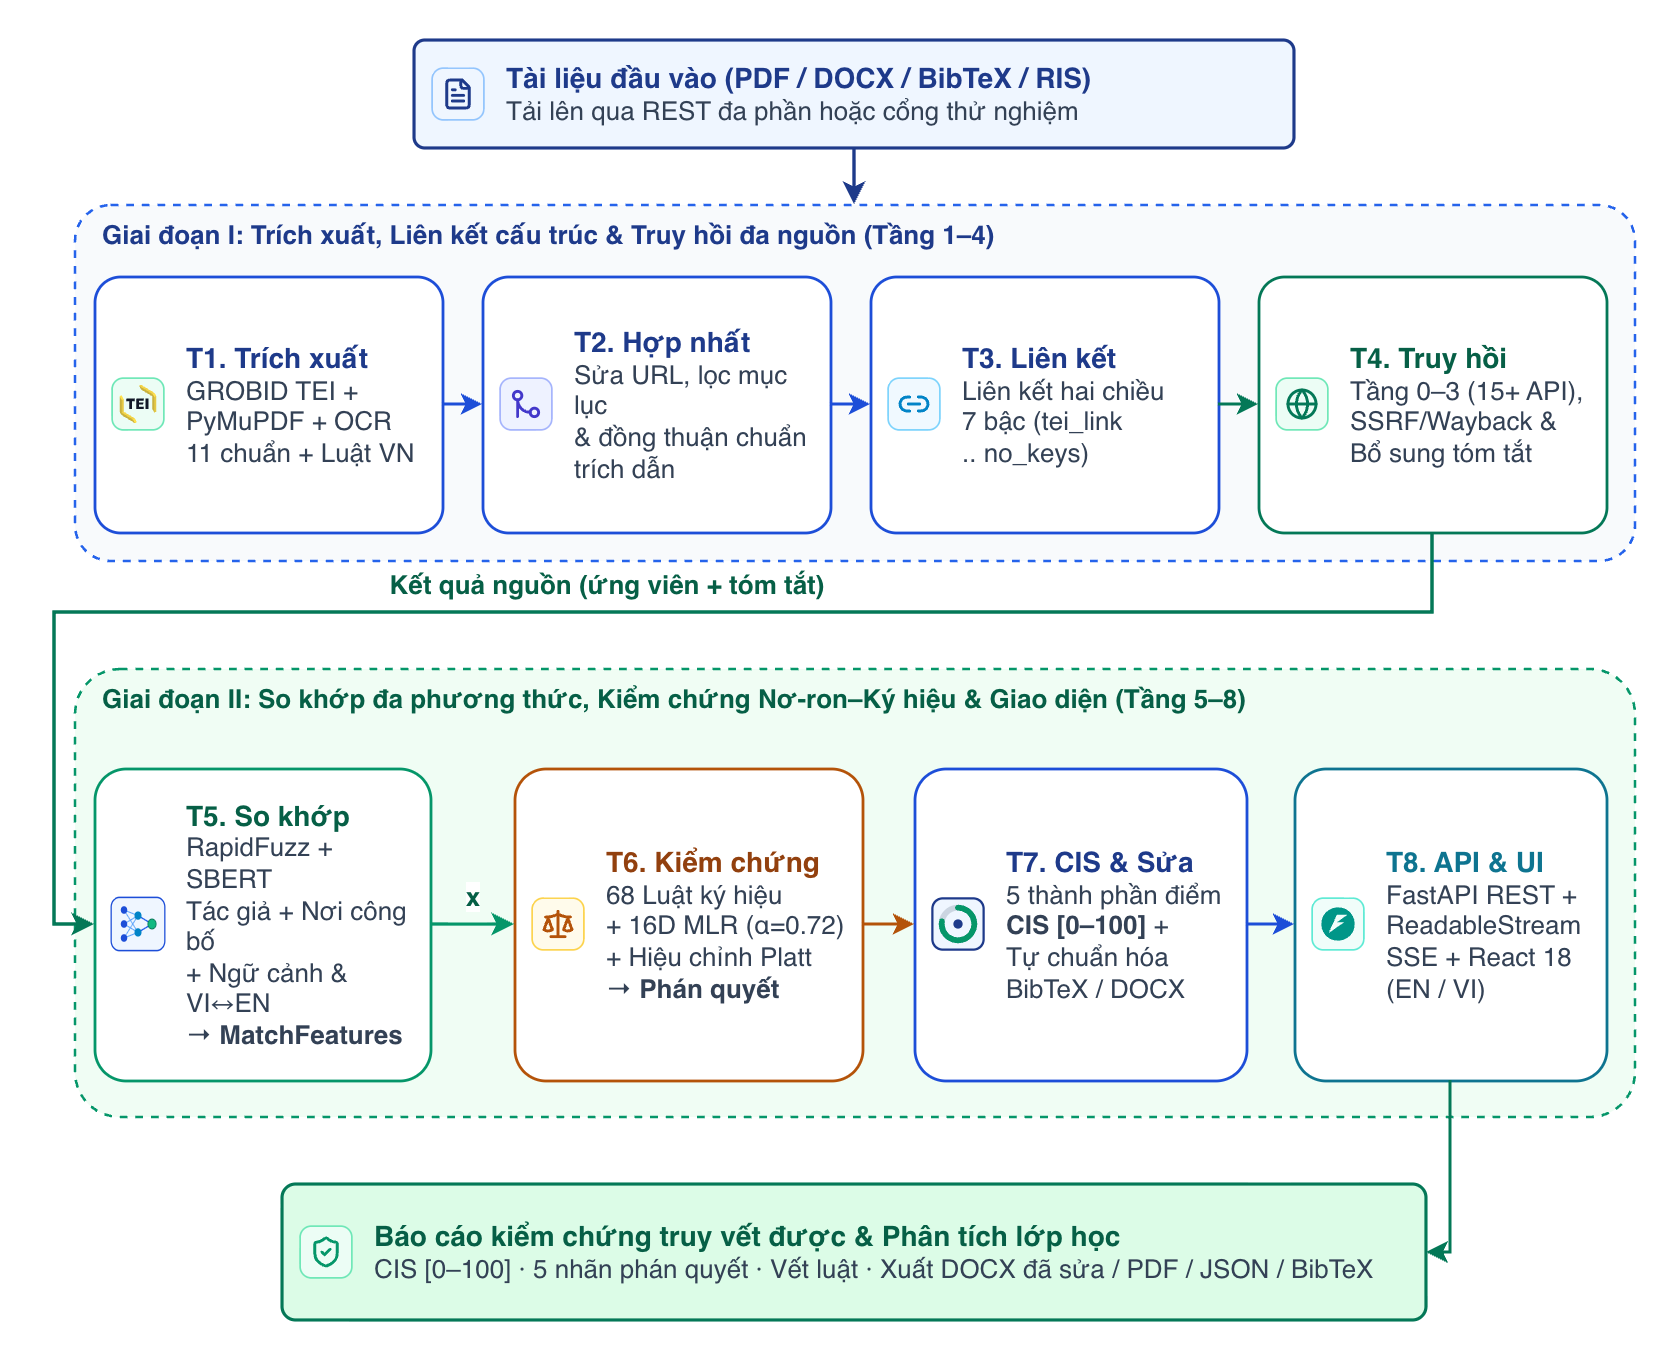
\includegraphics[width=\textwidth,keepaspectratio]{picture/figures/fig4_1_architecture.png}
    \caption[Kiến trúc phần mềm tám tầng và các hợp đồng suy giảm uyển chuyển]{Kiến trúc phần mềm tám tầng của CITRA (\texttt{v3.90.11}) thể hiện hợp đồng dữ liệu liên tầng và cơ chế suy giảm uyển chuyển.}
    \label{fig:architecture}
\end{figure}

Mỗi tầng đều tuân thủ một \emph{hợp đồng suy giảm uyển chuyển} nghiêm ngặt. Nếu container GROBID không phản hồi, Tầng 1 tự động chuyển sang phân tích hai cột bằng PyMuPDF và biểu thức chính quy. Nếu API trực tuyến trả mã HTTP 429 hoặc quá hạn, Tầng 4 sử dụng chỉ mục ngoại tuyến FTS5 129,137 bản ghi kèm cờ \texttt{api\_exhausted = True}, còn Tầng 6 định tuyến an toàn các ca thiếu bằng chứng sang \texttt{unresolved} thay vì phỏng đoán.

\subsection{Các mẫu thiết kế phần mềm}

Năm mẫu thiết kế hướng đối tượng và chịu lỗi đám mây duy trì tính mô-đun và khả năng bảo trì cho toàn bộ mã nguồn:
\begin{itemize}
    \item \textbf{Strategy và Priority Registry (\texttt{extraction/patterns/}):} Mười một bộ phân tích chuẩn trích dẫn quốc tế hiện thực giao thức \texttt{CitationFormat} theo mức ưu tiên số nguyên giảm dần ($100 \rightarrow 70$, giá trị lớn hơn được ưu tiên trước), kết hợp bộ trích xuất pháp luật Việt Nam chuyên biệt (\texttt{parse\_vn\_legal\_reference} / \texttt{VNLegalVerifier}) tạo thành mười hai định dạng hỗ trợ.
    \item \textbf{Adapter (\texttt{grobid\_adapter.py} \& các trình khách API):} Các định dạng ngoài không đồng nhất (GROBID TEI-XML, Crossref JATS XML, chỉ mục đảo OpenAlex, arXiv Atom XML và BibTeX) được chuẩn hóa về hai lớp đối tượng nội bộ thống nhất là \texttt{Citation} và \texttt{SourceCandidate}.
    \item \textbf{Chain of Responsibility (\texttt{CitationLinker} \& \texttt{SymbolicRules}):} Cả bộ liên kết bảy phương pháp lẫn bộ suy diễn ký hiệu 16 nhóm luật duyệt tuần tự chuỗi xử lý có thứ tự và ngắt mạch ngay khi điều kiện quyết định được thỏa mãn.
    \item \textbf{Bộ ngắt mạch (Circuit Breaker) và điều tiết tốc độ (\texttt{retrieval/}):} Mỗi trình khách API ngoài được bao bọc bởi máy trạng thái (\texttt{closed} $\rightarrow$ \texttt{open} $\rightarrow$ \texttt{half\_open}) và bộ điều tiết tốc độ bất đồng bộ (Token-Bucket hoặc đặt chỗ theo vòng lặp sự kiện) giúp bỏ qua tạm thời nhà cung cấp đang lỗi mà không làm tắc nghẽn các bài nộp khác.
    \item \textbf{Gộp yêu cầu đồng thời (Singleflight Request Coalescing):} Các truy vấn trùng khớp sau chuẩn hóa gửi đồng thời trong đợt tải lên hàng loạt dùng chung một coroutine HTTP duy nhất trước khi lưu vào bảng \texttt{citation\_cache}.
\end{itemize}

\section{Tầng trích xuất}

\subsection{Phân tích tài liệu đa định dạng}

Mô-đun tiếp nhận bản thảo (\texttt{DocumentParser}) hỗ trợ bốn định dạng: PDF, DOCX, BibTeX và RIS. Với tệp PDF, nhánh chính \texttt{grobid\_hybrid} gửi luồng nhị phân tới GROBID \texttt{0.9.1-crf}~\cite{Lopez2009} để tách đoạn thân bài, con trỏ nội văn \texttt{<ref type="bibr">}, cửa sổ câu ngữ cảnh và mục \texttt{<biblStruct>}. Hai bộ hậu xử lý tất định khắc phục nhiễu của đồ án sinh viên: (1)~\emph{bộ lọc mục lục (TOC) và dòng chấm dẫn} loại bỏ tiêu đề chương đánh số dễ nhầm thành mục tham khảo, và (2)~\emph{bước làm giàu bằng biểu thức chính quy} khôi phục URL, nhà xuất bản, số hiệu văn bản pháp luật Việt Nam và khoảng trang bị thẻ TEI-XML bỏ sót.

Khi GROBID tắt hoặc gặp bố cục phi chuẩn, \texttt{DocumentParser} chuyển sang đường ống dự phòng nhận biết hình học hai cột dựa trên PyMuPDF~\cite{PyMuPDF2024} và \texttt{pdfplumber}~\cite{Pdfplumber2024}. Trong \texttt{mupdf\_parser.py}, các trang có mật độ ký tự trích xuất gần bằng không tự động kích hoạt OCR Tesseract tiếng Việt/tiếng Anh có chọn lọc (bỏ qua cờ \texttt{fallback\_to\_ocr: false} mặc định trong \texttt{config.yaml} để đọc được PDF bản quét), còn các bảng mã tiếng Việt cũ (VNI, TCVN3) được chuẩn hóa về Unicode NFC. Tệp \texttt{.docx} gốc được đọc trực tiếp qua \texttt{python-docx} và thuộc tính đánh số XML không qua chuyển đổi trung gian.

Để triệt tiêu hiện tượng tráo trang bộ nhớ ảo trên máy chủ giới hạn tài nguyên (2 vCPU, $5.8\text{\,GiB}$ RAM), GROBID \texttt{0.9.1-crf}---với tập mô hình CRF Wapiti gốc chiếm khoảng $3.1\text{\,GiB}$ ngoài heap---khởi chạy qua \texttt{scripts/\allowbreak{}grobid-entrypoint.sh} trong container $4\text{\,GiB}$ với vùng nhớ JVM G1GC giới hạn chặt (\texttt{-Xmx768m} kèm \texttt{-XX:+ExitOnOutOfMemoryError}), \texttt{concurrency=2} (\texttt{poolMaxWait=30}), \texttt{modelPreload=true} và trần \texttt{pdfalto} $1{,}024\text{\,MB}$. Trên tuyến HTTP, \texttt{call\_grobid\_fulltext()} mặc định tắt tuần tự hóa hộp bao không dùng (\texttt{teiCoordinates}, hỗ trợ bật qua \texttt{GrobidConfig.tei\_coordinates} với khóa đệm \texttt{.coords-*}), tách thời gian chờ kết nối và đọc, dừng nhanh trước \texttt{ReadTimeout}/\texttt{SSLError} và chỉ thử lại sự cố kết nối tạm thời hoặc HTTP 502--504 bên ngoài semaphore đồng thời.

\subsection{Mười hai định dạng trích dẫn và nhận diện phong cách}

Các mục tham khảo và dấu trích dẫn nội văn được đối khớp trên mười một bản hiện thực giao thức \texttt{CitationFormat} xếp theo ưu tiên ($100 \rightarrow 70$) cùng bộ trích xuất văn bản pháp luật Việt Nam chuyên biệt tại Bảng~\ref{tab:styles} và Hình~\ref{fig:extraction}. Song song đó, \texttt{StyleDetector} thống kê cấu trúc toàn văn bản xuất ra \texttt{StyleProfile} (\texttt{APA-like}, \texttt{IEEE-like}, \texttt{MIXED} hoặc \texttt{UNKNOWN}); cờ pha trộn chuẩn \texttt{MIXED} chỉ bật khi có ít nhất hai họ chuẩn không tương thích cùng vượt $30\%$ và tổng số mục/dấu thỏa mãn $\text{total} \ge 5$.

{\setlength{\tabcolsep}{3.5pt}
\begin{longtable}{|L{0.16}|C{0.13}|L{0.32}|L{0.39}|}
\caption{Mười hai định dạng trích dẫn hỗ trợ (11 bản hiện thực \texttt{CitationFormat} và Pháp luật VN).}\label{tab:styles}\\
\hline
\textbf{Định dạng} & \textbf{Ưu tiên} & \textbf{Mẫu đánh dấu trong bài} & \textbf{Mẫu mục tài liệu tham khảo} \\
\hline
\endfirsthead
\multicolumn{4}{c}{\itshape Bảng \thetable\ (tiếp theo trang trước)}\\
\hline
\textbf{Định dạng} & \textbf{Ưu tiên} & \textbf{Mẫu đánh dấu trong bài} & \textbf{Mẫu mục tài liệu tham khảo} \\
\hline
\endhead
\hline
\multicolumn{4}{r}{\itshape Xem tiếp trang sau}\\
\endfoot
\hline
\endlastfoot
\textbf{APA (7th)} & \textbf{100} & \textit{(Author et al., 2020)}, \textit{Author (2020a)} & Author, A. B. (2020). Title of work. \textit{Venue, 12}(3), 45--67. \\
\hline
\textbf{IEEE} & \textbf{90} & \textit{[1]}, \textit{[1, 2]}, \textit{[1]--[3]} & [1] A. Author, ``Title,'' \textit{Venue}, vol.\ 1, pp.\ 1--10, 2020. \\
\hline
\textbf{ACM} & 88 & \textit{[1]}, \textit{[Author 2020]} & [1] Author Name. 2020. Title. In \textit{Proc.\ ACM}, 1--10. \\
\hline
\textbf{Harvard} & 85 & \textit{(Author, 2020)}, \textit{(Author 2020: 15)} & Author, A. (2020) \textit{Title}. Place: Publisher. \\
\hline
\textbf{Vancouver} & 80 & \textit{[1]}, \textit{(1--3)} & 1. Author AB. Title. \textit{Venue}. 2020;12(1):10--20. \\
\hline
\textbf{Nature} & 78 & Chỉ số trên / \textit{[1]} & 1. Author, A. Title. \textit{Nature} \textbf{580}, 100--105 (2020). \\
\hline
\textbf{CSE} & 77 & \textit{(Author 2020)}, chỉ số trên & Author AB. 2020. Title. \textit{Venue}. 12(1):10--20. \\
\hline
\textbf{ACS} & 76 & \textit{(1)}, chỉ số trên & (1) Author, A. B. Title. \textit{J.\ Am.\ Chem.\ Soc.} \textbf{2020}, \textit{142}, 1--5. \\
\hline
\textbf{AMA} & 75 & Chỉ số trên / \textit{[1]} & 1. Author AB. Title. \textit{JAMA}. 2020;323(1):1--10. \\
\hline
\textbf{Chicago} & 70 & \textit{(Author 2020, 45)}, chú thích chân trang & Author, First. 2020. \textit{Title}. Place: Publisher. \\
\hline
\textbf{MLA (9th)} & 70 & \textit{(Author 45)}, \textit{(Author and Coauthor 12)} & Author, First. ``Title.'' \textit{Venue}, vol.\ 1, no.\ 2, 2020, pp.\ 1--15. \\
\hline
\textbf{Pháp luật VN} & \textbf{Hàm riêng} & \textit{(Luật số 20/2023/QH15)} & Quốc hội / Chính phủ. (2023). \textit{Luật / Nghị định / Thông tư}. \\
\hline
\end{longtable}
}

\begin{figure}[!htbp]
    \centering
    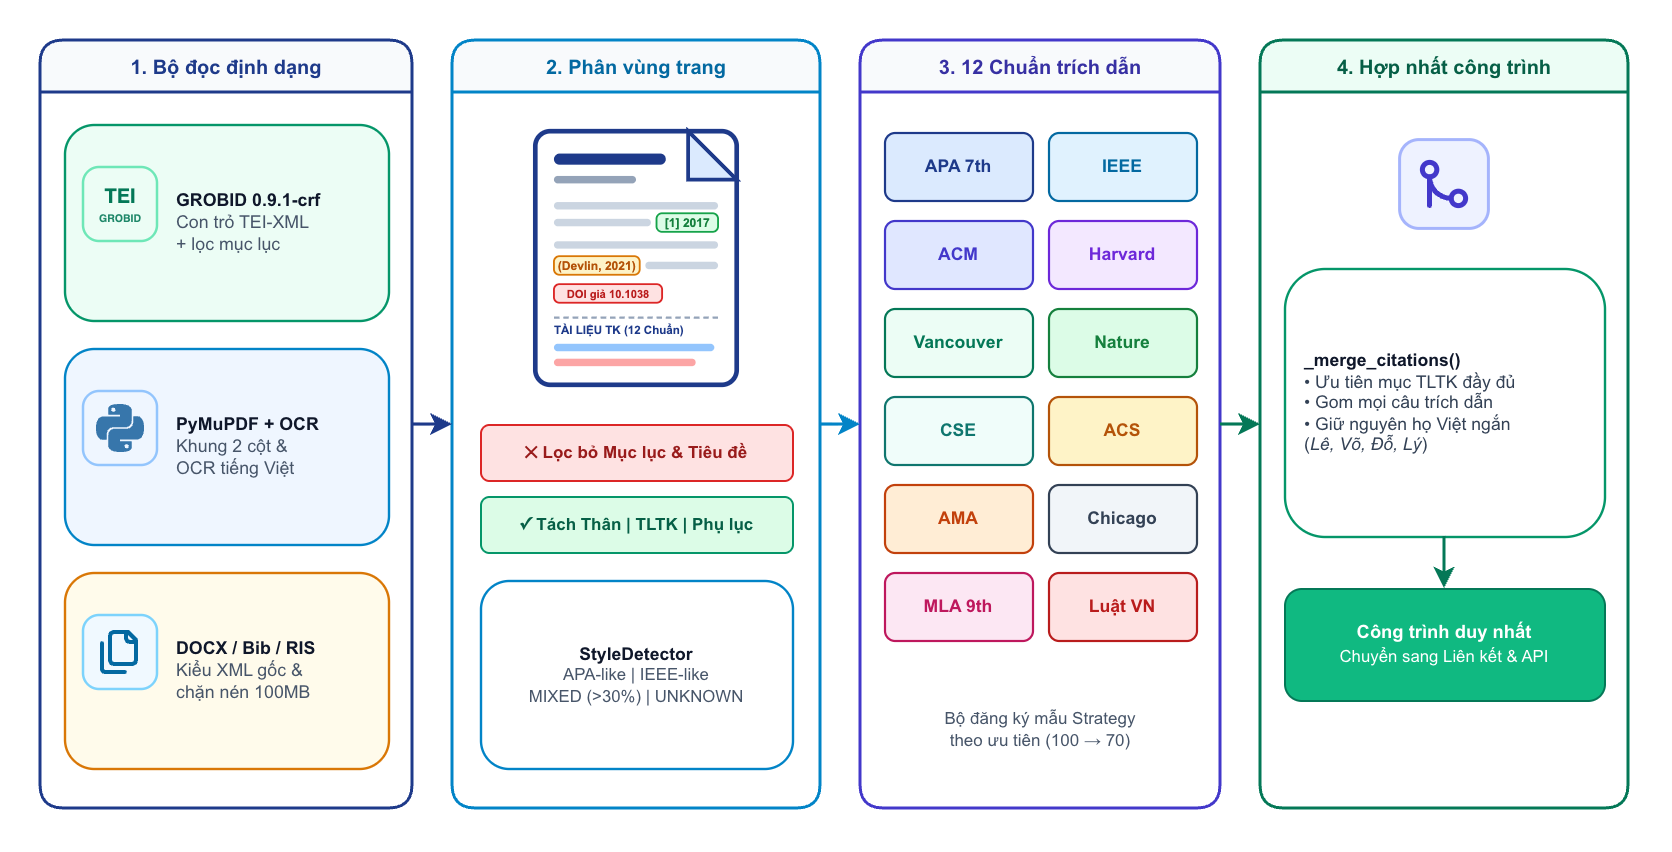
\includegraphics[width=\textwidth,keepaspectratio]{picture/figures/fig4_2_extraction.png}
    \caption[Đường ống trích xuất đa định dạng cho PDF, DOCX, BibTeX và RIS]{Kiến trúc tầng trích xuất kết hợp GROBID \texttt{0.9.1-crf} TEI-XML, bộ lọc mục lục (TOC), dự phòng PyMuPDF hai cột, OCR chọn lọc và mười hai định dạng trích dẫn.}
    \label{fig:extraction}
\end{figure}

\section{Hợp nhất và liên kết hai chiều}

\subsection{Hợp nhất trích dẫn ở mức công trình}

Tầng trích xuất trả về dấu trích dẫn nội văn, danh mục tài liệu tham khảo và trích dẫn phụ lục. Phương thức \texttt{IntegrityPipeline.\_merge\_citations} hợp nhất các bản ghi tương ứng thành tập công trình duy nhất nhưng vẫn gắn đầy đủ mọi vị trí xuất hiện nội văn làm quan sát ngữ cảnh. Các họ tiếng Việt hai ký tự (\textit{Le}, \textit{Vo}, \textit{Do}, \textit{Ho}, \textit{Ly}) được bảo toàn tường minh trong chuẩn hóa họ tên để không bị cắt nhầm thành chữ viết tắt. Các cụm gộp như \texttt{[9, 10]} hay \textit{(Vaswani et al., 2017; Devlin et al., 2019)} được tách phẳng thành từng cạnh độc lập, còn mục đánh số gộp (\texttt{[14] a) ... b) ...}) tách thành mục con (\texttt{14a}, \texttt{14b}).

\subsection{Bộ liên kết bảy phương pháp, thuật toán hình thức và trạng thái ánh xạ}

Tính toàn vẹn cấu trúc đòi hỏi đồ thị hai phía nhất quán giữa nhận định trong bài và danh mục tham khảo. Như hình thức hóa tại Thuật toán~\ref{alg:linker} và minh họa ở Hình~\ref{fig:linking}, \texttt{CitationLinker} thực thi thác bảy phương pháp tự động theo đúng thứ tự thực thi (Bảng~\ref{tab:mapping-methods}, trong đó \texttt{numeric\_index} chạy trước \texttt{author\_year}, kèm \texttt{manual\_review} khi giảng viên ghi đè) và gán một trong tám nhãn \texttt{MappingStatus} (Bảng~\ref{tab:mapping-statuses}). Mục tham khảo trùng lặp được nhận diện sau bước liên kết qua khớp chính xác DOI/arXiv hoặc độ tương đồng gộp tiêu đề -- tác giả -- năm $\ge 0.92$ và loại khỏi tập chưa trích dẫn để tránh phạt kép. Khi xảy ra \texttt{ambiguous\_mapping}, bộ liên kết gắn ứng viên đồng hạng đầu tiên với $\text{conf} = 0.50$ và tầng kiểm chứng phía sau trả về \texttt{unresolved}.

\begin{citraalgo}{4.1}{\texttt{BidirectionalCitationLink}$(\mathcal{M}, \mathcal{B})$}{alg:linker}
\textbf{Đầu vào:} Dấu trích dẫn nội văn $\mathcal{M} = \{m_1, \dots, m_k\}$, danh mục tham khảo $\mathcal{B} = \{r_1, \dots, r_N\}$.\\
\textbf{Đầu ra:} Tập liên kết $\mathcal{L}$, tập mục không được trích dẫn $\mathcal{U} \subseteq \mathcal{B}$, các cặp trùng lặp $\mathcal{D}$.
{\setlength{\leftmargini}{1.6em}
\begin{enumerate}\setlength{\itemsep}{1pt}\setlength{\parskip}{0pt}
\item Dựng các chỉ mục tra cứu trên $\mathcal{B}$: $I_{\text{tei}}$ (\texttt{xml:id}), $I_{\text{doi}}$ (DOI chuẩn hóa), $I_{\text{arxiv}}$ (mã arXiv chuẩn), $I_{\text{num}}$ (số thứ tự) và $I_{\text{ay}}$ (họ tác giả, năm, hậu tố).
\item $\mathcal{L} \leftarrow \emptyset$; $\mathcal{C}_{\text{cited}} \leftarrow \emptyset$.
\item \textbf{với mỗi} $m \in \mathcal{M}$ \textbf{thực hiện}
\item \quad Tra cứu theo thứ tự ưu tiên nghiêm ngặt: (a)~$I_{\text{tei}}[m]$ ($0.98$); (b)~$I_{\text{doi}}[m]$ ($0.95$); (c)~$I_{\text{arxiv}}[m]$ ($0.95$); (d)~$I_{\text{num}}[m]$ ($0.90$); (e)~$I_{\text{ay}}[m]$ ($0.90$); (f)~khớp mờ Jaccard tập từ / \texttt{difflib} $s \ge \tau_{\text{fuzz}} = 0.80$ ($\text{conf} = 0.65\,s$).
\item \quad \textbf{nếu} tìm thấy duy nhất đích $r^*$ \textbf{thì} đặt $\text{status} \leftarrow \texttt{in\_text\_mismatch}$ nếu $m$ và $r^*$ lệch năm/họ, ngược lại \texttt{matched}; thêm $(m, r^*, \text{status})$ vào $\mathcal{L}$ và $r^*$ vào $\mathcal{C}_{\text{cited}}$.
\item \quad \textbf{ngược lại nếu} có nhiều đích đồng hạng $\{r_1, r_2, \dots\}$ \textbf{thì} ghi $(m, r_j, \texttt{ambiguous\_mapping}, \text{conf}=0.50)$ cho mỗi $r_j$ đồng hạng (hoặc $r_1$ ở mức $0.65\,s$ khi đồng hạng mờ) vào $\mathcal{L}$.
\item \quad \textbf{ngược lại} ghi $(m, \bot, \texttt{missing\_reference}, \text{method}=\texttt{no\_keys}, \text{conf}=0.0)$ vào $\mathcal{L}$.
\item Phát hiện các cặp trùng lặp $\mathcal{D} \leftarrow \texttt{DuplicateDetector}(\mathcal{B})$ (khớp DOI/arXiv hoặc tương đồng $\ge 0.92$) và loại bản sao phụ $\mathcal{D}_{\text{non-canon}}$ khỏi diện phạt chưa trích dẫn.
\item $\mathcal{U} \leftarrow (\mathcal{B} \setminus \mathcal{C}_{\text{cited}}) \setminus \mathcal{D}_{\text{non-canon}}$ (gán nhãn \texttt{uncited\_reference}); \textbf{trả về} $(\mathcal{L}, \mathcal{U}, \mathcal{D})$.
\end{enumerate}}
\end{citraalgo}

\begin{figure}[!htbp]
    \centering
    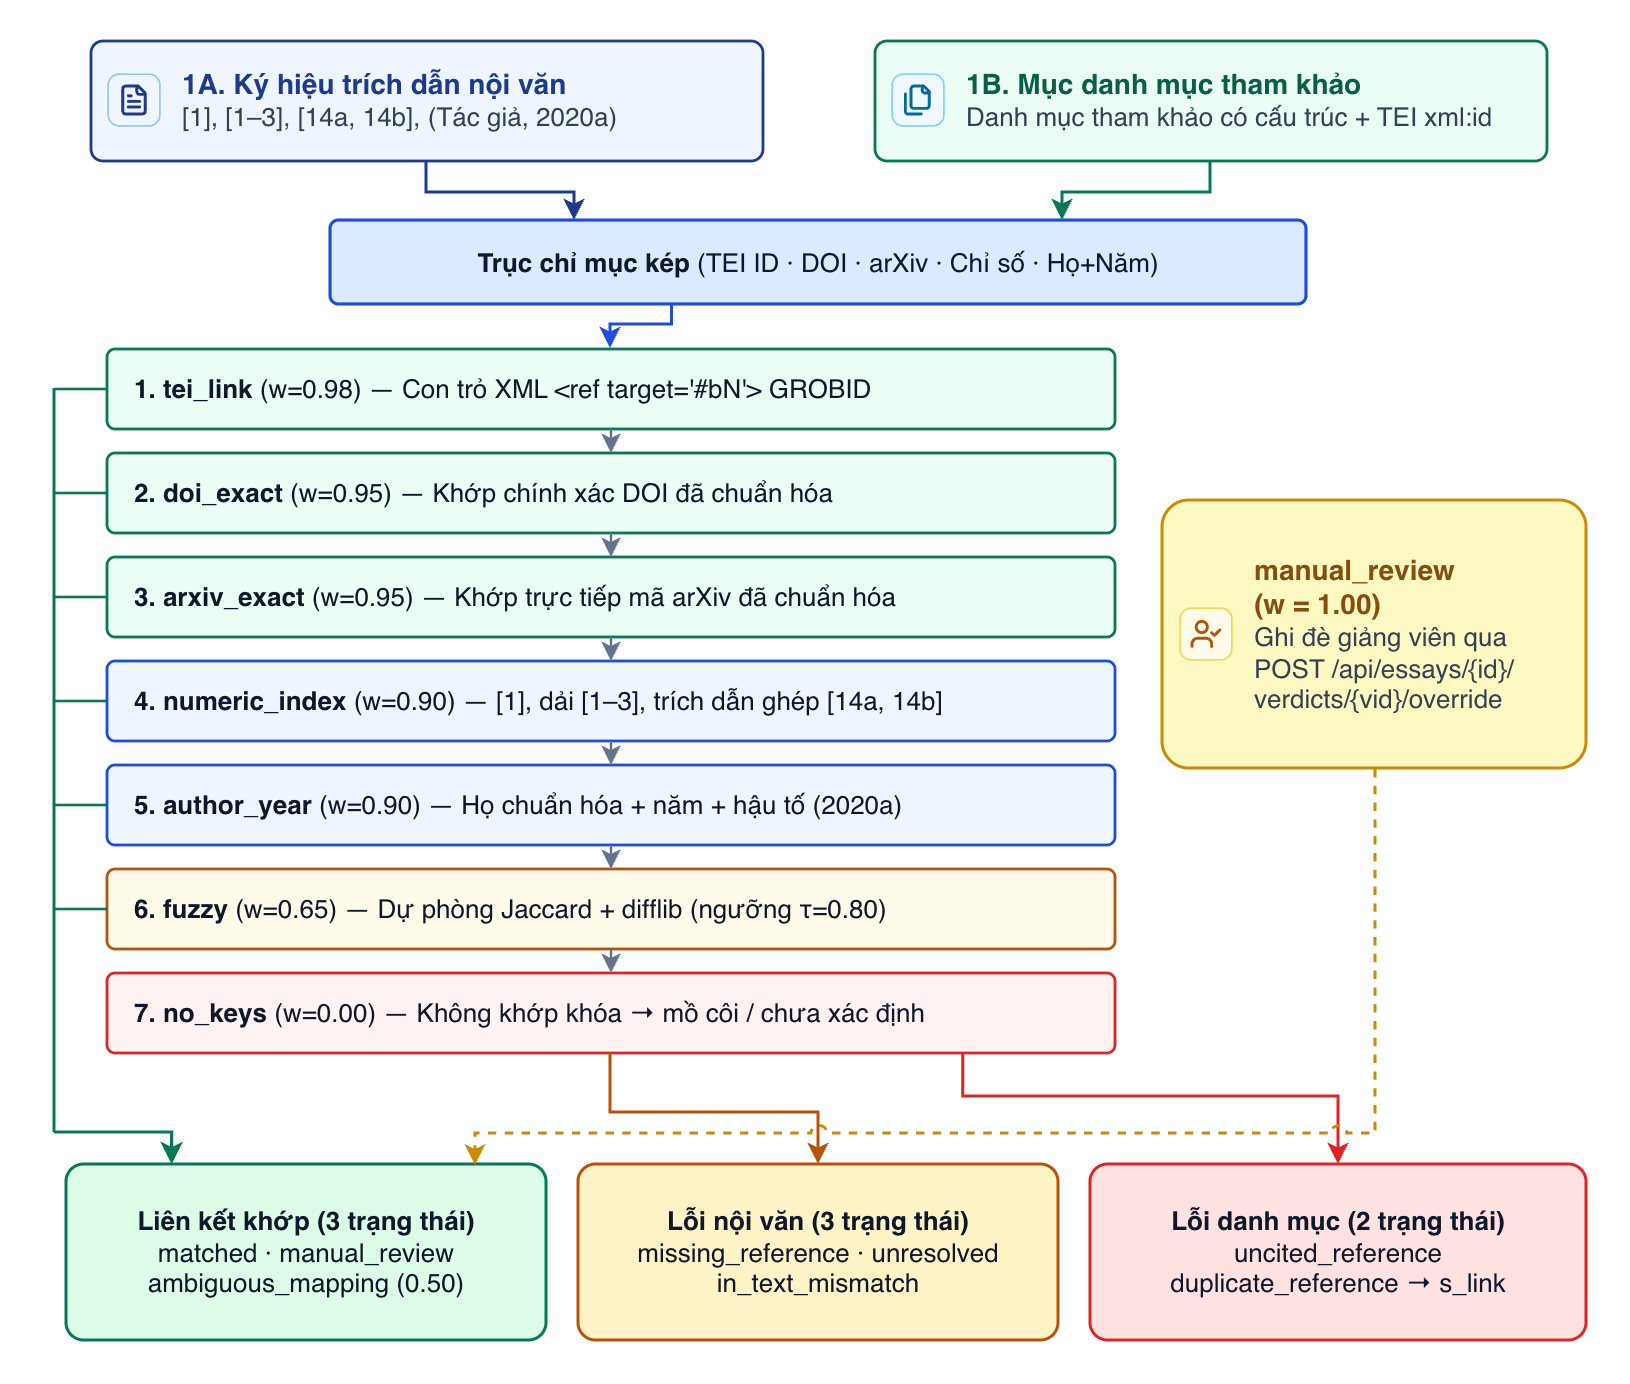
\includegraphics[width=\textwidth,keepaspectratio]{picture/figures/fig4_3_linking.png}
    \caption[Thác phân giải liên kết hai chiều bảy phương pháp và tám trạng thái ánh xạ]{Thác liên kết trích dẫn hai chiều qua bảy phương pháp phân giải tự động (đúng thứ tự thực thi mã nguồn) và tám trạng thái ánh xạ cấu trúc tương ứng.}
    \label{fig:linking}
\end{figure}
\FloatBarrier

{\setlength{\tabcolsep}{3.5pt}
\begin{longtable}{|L{0.25}|C{0.15}|L{0.60}|}
\caption[Thứ tự phương pháp phân giải trong \texttt{CitationLinker}]{Các phương pháp phân giải theo đúng thứ tự ưu tiên trong \texttt{CitationLinker}.}\label{tab:mapping-methods}\\
\hline
\textbf{Phương pháp} & \textbf{Độ tin cậy} & \textbf{Tiêu chí đối sánh} \\
\hline
\endfirsthead
\multicolumn{3}{c}{\itshape Bảng \thetable\ (tiếp theo trang trước)}\\
\hline
\textbf{Phương pháp} & \textbf{Độ tin cậy} & \textbf{Tiêu chí đối sánh} \\
\hline
\endhead
\hline
\multicolumn{3}{r}{\itshape Xem tiếp trang sau}\\
\endfoot
\hline
\endlastfoot
\textbf{\texttt{tei\_link}} & \textbf{0.98} & Con trỏ trực tiếp \texttt{xml:id} trong GROBID TEI-XML nối từ \texttt{<ref>} tới \texttt{<biblStruct>}. \\
\hline
\textbf{\texttt{doi\_exact}} & \textbf{0.95} & Mã DOI chuẩn hóa trùng khớp ở cả dấu trích dẫn nội văn và mục tài liệu tham khảo. \\
\hline
\textbf{\texttt{arxiv\_exact}} & \textbf{0.95} & Định danh chuẩn \texttt{arXiv} trích xuất trùng khớp ở cả hai phía. \\
\hline
\textbf{\texttt{numeric\_index}} & 0.90 & Số thứ tự ngoặc vuông hoặc chỉ số trên (hoặc dải \texttt{[1]--[3]}) khớp chỉ mục tài liệu tham khảo. \\
\hline
\textbf{\texttt{author\_year}} & 0.90 & Họ tác giả chuẩn hóa, năm xuất bản và hậu tố (\texttt{a}--\texttt{f}) đồng nhất (gồm suy diễn MLA). \\
\hline
\textbf{\texttt{fuzzy}} & 0.65 & Chồng lấn từ khóa tiêu đề hoặc tác giả vượt ngưỡng dự phòng khi thiếu khóa định danh. \\
\hline
\textbf{\texttt{no\_keys}} & \textbf{0.00} & Độ tin cậy thực thi khi thiếu khóa phân biệt (\texttt{missing\_reference}; giá trị enum mặc định $0.30$ khi chưa ghi đè). \\
\hline
\textbf{\texttt{manual\_review}} & \textbf{1.00} & Liên kết được giảng viên có thẩm quyền ghi đè trực tiếp (\texttt{api/routes/verdicts.py}). \\
\hline
\end{longtable}
}

{\setlength{\tabcolsep}{3.5pt}
\begin{longtable}{|L{0.28}|C{0.15}|C{0.14}|L{0.43}|}
\caption{Tám trạng thái ánh xạ cấu trúc và mức phạt tương ứng trong thang điểm CIS.}\label{tab:mapping-statuses}\\
\hline
\textbf{Trạng thái ánh xạ} & \textbf{Lỗi toàn vẹn} & \textbf{Mức phạt CIS} & \textbf{Ý nghĩa cấu trúc} \\
\hline
\endfirsthead
\multicolumn{4}{c}{\itshape Bảng \thetable\ (tiếp theo trang trước)}\\
\hline
\textbf{Trạng thái ánh xạ} & \textbf{Lỗi toàn vẹn} & \textbf{Mức phạt CIS} & \textbf{Ý nghĩa cấu trúc} \\
\hline
\endhead
\hline
\multicolumn{4}{r}{\itshape Xem tiếp trang sau}\\
\endfoot
\hline
\endlastfoot
\textbf{\texttt{matched}} & Không & 0.00 & Liên kết một--một duy nhất, nhất quán về tác giả và năm xuất bản. \\
\hline
\textbf{\texttt{missing\_reference}} & \textbf{Có} & \textbf{0.20} & Dấu trích dẫn trong bài viện dẫn nguồn không có trong danh mục (trích dẫn mồ côi). \\
\hline
\textbf{\texttt{in\_text\_mismatch}} & \textbf{Có} & \textbf{0.15} & Cặp đã liên kết mâu thuẫn nhau về năm xuất bản, họ tác giả hoặc từ khóa tiêu đề. \\
\hline
\textbf{\texttt{uncited\_reference}} & \textbf{Có} & \textbf{0.10} & Mục tài liệu tham khảo liệt kê cuối bài nhưng không được trích dẫn trong nội dung. \\
\hline
\textbf{\texttt{duplicate\_reference}} & \textbf{Có} & \textbf{0.10} & Hai hoặc nhiều mục trong danh mục cùng trỏ về một ấn phẩm duy nhất. \\
\hline
\textbf{\texttt{ambiguous\_mapping}} & \textbf{Có} & 0.05 & Dấu trích dẫn nội văn khớp đồng hạng với nhiều mục tài liệu tham khảo. \\
\hline
\textbf{\texttt{style\_inconsistent}} & \textbf{Có} & 0.02 & Mục tham khảo hoặc dấu trích dẫn lệch khỏi chuẩn chủ đạo của bản thảo. \\
\hline
\textbf{\texttt{unresolved}} & Không & 0.00 & Không đủ thông tin cấu trúc để phân loại trạng thái liên kết. \\
\hline
\end{longtable}
}

\section{Truy hồi liên hợp và kiểm chứng URL}

\subsection{Điều phối bốn tầng nhận biết miền tri thức}

Thay vì phát tán mọi mục tham khảo tới toàn bộ API ngoài, \texttt{Retrieval\allowbreak Orchestrator} định tuyến truy vấn qua kiến trúc bốn tầng ở Hình~\ref{fig:retrieval}:
\begin{enumerate}
    \item \textbf{Tiền sàng lọc (Pre-Screening):} URL thuần web, kho phần mềm, chuẩn IETF RFC, gói PyPI, thẻ Hugging Face và văn bản pháp luật Việt Nam (\texttt{parse\_vn\_legal\_reference} + \texttt{VNLegalVerifier}) đi thẳng tới bộ kiểm chứng kỹ thuật/pháp lý chuyên biệt.
    \item \textbf{Tầng 0 (Tra cứu ngoại tuyến dưới 100\,ms):} Kiểm tra danh sách trắng 101 công trình kinh điển (\texttt{\_KNOWN\_PAPERS}) và chỉ mục SQLite FTS5 cục bộ (\texttt{local\_papers.db}, 129,137 bản ghi; 128,115 bài báo duy nhất; 82,887 tóm tắt; $98.42\%$ ACL Anthology) bằng Okapi BM25~\cite{robertson2009bm25}.
    \item \textbf{Tầng 1 (Các cơ sở dữ liệu công khai cốt lõi):} Dựa vào dấu hiệu DOI, arXiv, ISBN hoặc tiêu đề, các truy vấn bất đồng bộ chạy dưới giới hạn tốc độ cấu hình tới \textbf{Crossref} ($25\text{\,req/s}$ polite pool + Retraction Watch), \textbf{OpenAlex} ($8\text{\,req/s}$), \textbf{DataCite} và \textbf{Global DOI RA} (kèm thăng hạng Tầng~1 theo dấu hiệu chuyên ngành cho arXiv, DBLP, Europe PMC hoặc DOAJ/OpenAIRE).
    \item \textbf{Tầng 2 (Chuyên ngành \& Pha 2.5 làm giàu arXiv):} Định tuyến theo lĩnh vực tới \textbf{DOAJ}, \textbf{OpenAIRE/HAL}, \textbf{DBLP} ($1.5\text{\,req/s}$), \textbf{Europe PMC} ($5.0\text{\,req/s}$), \textbf{NCBI/bioRxiv}, \textbf{OpenLibrary / Google Books} ($3.0\text{\,req/s}$), \textbf{Wikidata / OpenCitations}, \textbf{IETF RFC / PyPI / Hugging Face} và Pha 2.5 \textbf{arXiv API} (giãn cách đặt chỗ tuần tự $1.0\text{\,s}$). Khi ứng viên tốt nhất khuyết bản tóm tắt, \texttt{\_enrich\_missing\_abstract} truy vấn tối đa ba nguồn ưu tiên hàng đầu (\texttt{pool[:3]}) trong tập chín bộ chuyển đổi làm giàu để chặn độ trễ đuôi.
    \item \textbf{Tầng 3 (Dự phòng tìm kiếm web tùy chọn):} Truy vấn không có ứng viên có thể tùy chọn gọi \textbf{Serper / SerpAPI} chỉ khi đơn vị vận hành cấu hình khóa API riêng.
\end{enumerate}

\begin{figure}[!htbp]
    \centering
    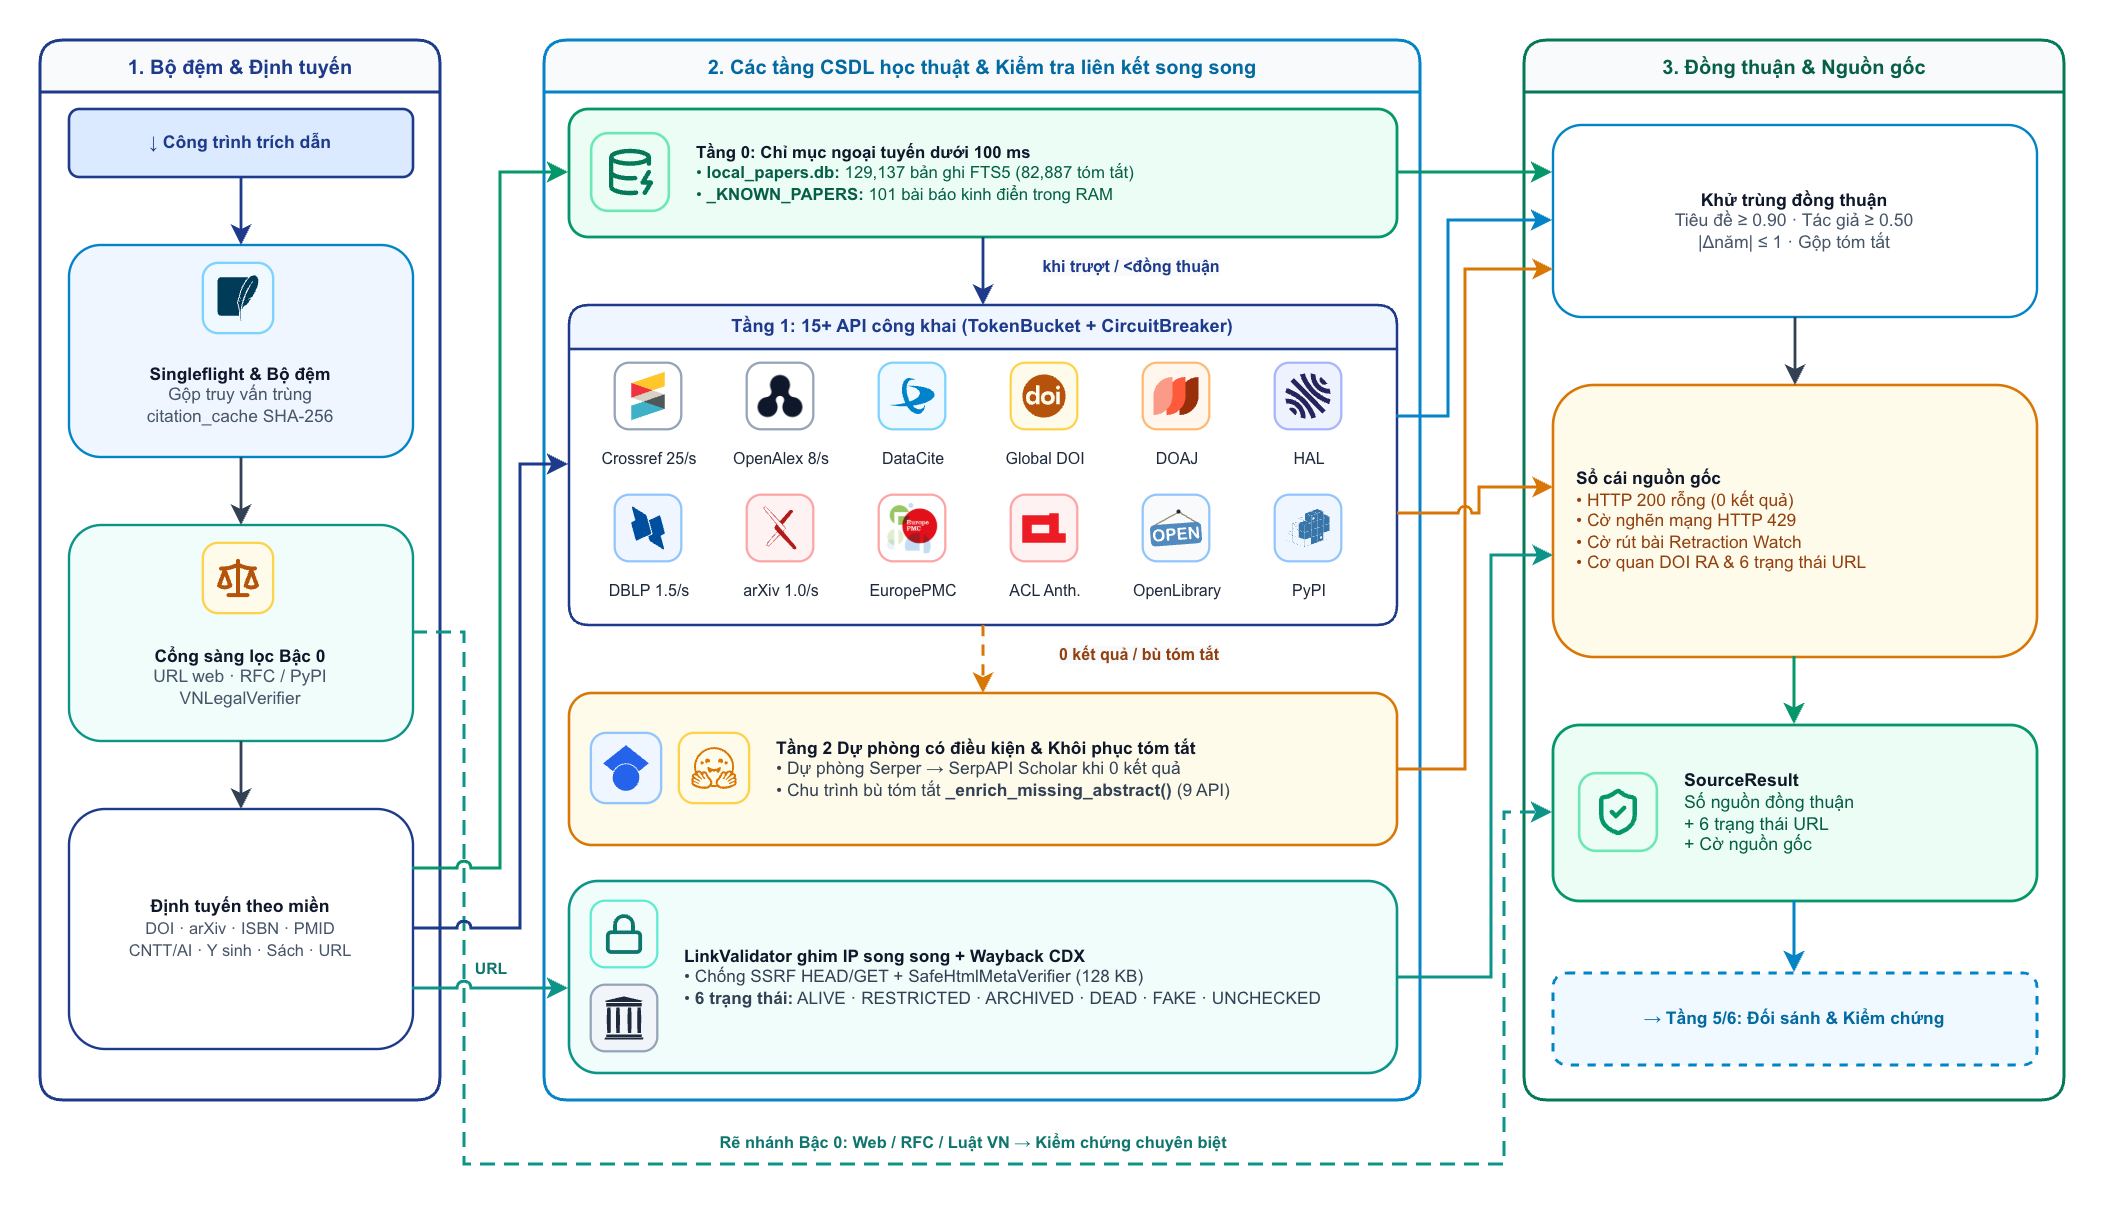
\includegraphics[width=\textwidth,keepaspectratio]{picture/figures/fig4_4_retrieval.png}
    \caption[Truy hồi bốn tầng nhận biết miền tri thức và kiểm tra URL chống SSRF]{Điều phối truy hồi bốn tầng qua Tầng 0 (SQLite FTS5 + 101 công trình kinh điển), Tầng 1 (API công khai cốt lõi), Tầng 2 (Chuyên ngành \& arXiv), Tầng 3 (Tìm kiếm tùy chọn) và kiểm chứng song song HTTP/Wayback/HTML.}
    \label{fig:retrieval}
\end{figure}

\subsection[Đồng thuận đa nguồn, bảo vệ SSRF và SafeHtmlMetaVerifier]{Đồng thuận đa nguồn, bộ bảo vệ SSRF ghim IP và SafeHtmlMetaVerifier}
\label{sec:consensus}

Các ứng viên trả về được khử trùng lặp và chấm điểm đồng thuận đa nguồn (\texttt{title\_sim} $\ge 0.90$, \texttt{author\_jaccard} $\ge 0.50$, $|\Delta y| \le 1$), kế thừa chéo bản tóm tắt giữa các cơ sở dữ liệu nhất trí. Song song đó, \texttt{LinkValidator} thăm dò URL trích dẫn và ảnh chụp Internet Archive Wayback CDX~\cite{wayback-cdx}, gán một trong \textbf{sáu trạng thái \texttt{LinkStatus}}: \texttt{alive} (HTTP 200--399), \texttt{restricted\_alive} (HTTP 401/403/405/429 chống bot/tường phí), \texttt{archived\_alive} (khôi phục qua Wayback), \texttt{dead\_link} (HTTP 404/410 hoặc NXDOMAIN), \texttt{fake\_domain} (tên miền giữ chỗ theo RFC 2606~\cite{rfc2606}) hoặc \texttt{unchecked}. Với tài nguyên web truy cập được, \texttt{SafeHtmlMetaVerifier} đọc tối đa $128\text{\,KB}$ đầu trang (\texttt{MAX\_HTML\_HEAD\_BYTES = 131,072}) để bóc tách siêu dữ liệu Highwire Press, Dublin Core, OpenGraph và JSON-LD đồng thời phát hiện trang lỗi ``Soft-404'' song ngữ Anh/Việt dưới mã HTTP 200.

Để ngăn chặn tấn công DNS rebinding và dò quét mạng nội bộ, toàn bộ kết nối URL đi ra đều đi qua \texttt{SSRFSafeAsyncNetworkBackend} (định nghĩa trong \texttt{retrieval/html\_meta\_verifier.py} và dùng chung bởi \texttt{link\_validator.py} cùng \texttt{SafeHtmlMetaVerifier}). Trước khi mở socket, tầng truyền tải phân giải toàn bộ bản ghi A/AAAA qua \texttt{socket.getaddrinfo}, chỉ cho phép cổng $\{80, 443\}$ và lập tức từ chối nếu \emph{bất kỳ} địa chỉ IP nào rơi vào vùng loopback, link-local, mạng riêng RFC 1918, IPv4 ánh xạ IPv6 (\texttt{::ffff:127.0.0.1}) hoặc siêu dữ liệu đám mây (\texttt{169.254.169.254}). Bên trong \texttt{connect\_tcp()}, tầng truyền tải kết nối thẳng vào chuỗi IP đã xác minh đồng thời giữ nguyên tên miền gốc cho TLS Server Name Indication (SNI) và tiêu đề HTTP \texttt{Host} nhằm bảo toàn xác thực chứng chỉ X.509, đồng thời lặp lại toàn bộ quy trình kiểm tra DNS/IP trên từng bước chuyển hướng HTTP 3xx.

\section{Đối sánh từ vựng, nơ-ron và xuyên ngôn ngữ}

\subsection{Đối sánh từ vựng và trường thư mục}

Từ đối tượng \texttt{SourceCandidate} tốt nhất, \texttt{FeatureCalculator} tính tập tín hiệu \texttt{MatchFeatures} tại Bảng~\ref{tab:features}. Ba bộ chuẩn hóa miền học thuật loại bỏ cảnh báo siêu dữ liệu giả: tách tiêu đề phụ sau dấu hai chấm/lần tái bản cấp mức tương đồng $0.95$ cho tiền tố tiêu đề chính khớp sạch; đối chiếu arXiv -- kỷ yếu lấy $|\Delta y|$ nhỏ nhất giữa bản tiền ấn phẩm và bản xuất bản chính thức; và \texttt{VenueNormalizer} mở rộng bí danh hội nghị/tạp chí (\texttt{NeurIPS} $\leftrightarrow$ \texttt{Advances in Neural Information Processing Systems}).

{\setlength{\tabcolsep}{3.5pt}
\begin{longtable}{|L{0.28}|C{0.12}|L{0.60}|}
\caption{Các đặc trưng đối sánh chính do \texttt{FeatureCalculator} và \texttt{LinkValidator} tính toán.}\label{tab:features}\\
\hline
\textbf{Tên đặc trưng} & \textbf{Kiểu} & \textbf{Cách tính toán} \\
\hline
\endfirsthead
\multicolumn{3}{c}{\itshape Bảng \thetable\ (tiếp theo trang trước)}\\
\hline
\textbf{Tên đặc trưng} & \textbf{Kiểu} & \textbf{Cách tính toán} \\
\hline
\endhead
\hline
\multicolumn{3}{r}{\itshape Xem tiếp trang sau}\\
\endfoot
\hline
\endlastfoot
\textbf{\texttt{title\_sim\_fuzzy}} & \texttt{float} & Giá trị lớn nhất giữa khớp chính xác, khớp tiền tố tiêu đề chính ($0.95$), chuỗi con có kiểm soát ($0.90$) và RapidFuzz \texttt{token\_set\_ratio}. \\
\hline
\textbf{\texttt{title\_sim\_semantic}} & \texttt{float} & Độ tương đồng cosine giữa véc-tơ nhúng \texttt{all-MiniLM-L6-v2} của tiêu đề trích dẫn và tiêu đề ứng viên. \\
\hline
\textbf{\texttt{title\_sim\_max}} & \texttt{float} & Giá trị lớn nhất giữa \texttt{title\_sim\_fuzzy} và \texttt{title\_sim\_semantic}. \\
\hline
\textbf{\texttt{author\_jaccard}} & \texttt{float} & Chồng lấn họ tác giả đã lược dấu nhưng bảo toàn các họ tiếng Việt ngắn (\textit{Le}, \textit{Vo}, \textit{Do}, \textit{Ho}, \textit{Ly}). \\
\hline
\textbf{\texttt{year\_distance}} & \texttt{int} & Giá trị nhỏ nhất $|y_{\text{cited}} - y_{\text{cand}}|$ giữa các bản ghi tiền ấn phẩm/tái bản ($999$ nếu khuyết năm). \\
\hline
\textbf{\texttt{venue\_sim}} & \texttt{float} & Độ tương đồng từ khóa nơi công bố trong $[0, 1]$ sau mở rộng bí danh bởi \texttt{VenueNormalizer}. \\
\hline
\textbf{\texttt{doi\_exact\_match}} & \texttt{bool} & Khớp chính xác mã DOI chuẩn hóa hoặc tương đương chuẩn giữa DOI arXiv và DOI nhà xuất bản. \\
\hline
\textbf{\texttt{source\_consensus}} & \texttt{int} & Số lượng cơ sở dữ liệu độc lập cùng trả về bản ghi ứng viên củng cố nhau. \\
\hline
\textbf{\texttt{content\_alignment\_score}} & \texttt{float} & Điểm căn chỉnh nơ-ron gộp theo câu giữa ngữ cảnh trích dẫn và tiêu đề/tóm tắt ứng viên (Phương trình~\eqref{eq:abs-pooling}). \\
\hline
\textbf{\texttt{stance\_label}} & \texttt{str} & Nhãn lập trường hỗ trợ (\texttt{supported}, \texttt{partially\_supported}, \texttt{neutral}, \texttt{contradiction\_risk}) qua lọc độ đặc trưng gốc từ. \\
\hline
\textbf{\texttt{url\_status}} & \texttt{enum} & Trạng thái hoạt động sáu mức của URL (\texttt{alive}, \texttt{restricted\_alive}, \texttt{archived\_alive}, \texttt{dead\_link}, \texttt{fake\_domain}, \texttt{unchecked}). \\
\hline
\end{longtable}
}

\subsection{Căn chỉnh ngữ nghĩa bằng bộ mã hóa kép và phân tích lập trường}

Hình~\ref{fig:matching} minh họa đường ống bộ mã hóa kép trong \texttt{SemanticMatcher}. Các nhận định và bản tóm tắt đơn ngữ tiếng Anh được mã hóa bằng Sentence-BERT (\texttt{all-MiniLM-L6-v2}, 384D)~\cite{reimers2019sbert} và gộp theo câu bằng Phương trình~\eqref{eq:abs-pooling} ($0.65\,\max + 0.35\,\mathrm{abs}$, thống nhất trên cả nhánh chạy lô lẫn nhánh dự phòng từng câu), tổng hợp tối đa tám vị trí trích dẫn mỗi công trình. Khi phát hiện văn bản song ngữ Việt -- Anh theo bất kỳ chiều nào (\texttt{VI}$\leftrightarrow$\texttt{EN}), \texttt{SemanticMatcher} tự động gọi bộ mã hóa lượng tử hóa ONNX INT8 \texttt{paraphrase-multilingual-MiniLM-L12-v2}~\cite{reimers2020multilingual}, bổ trợ bằng từ điển bắc cầu học thuật (\texttt{vn\_en\_academic\_bridge}) và áp dụng mức bù tương đồng xuyên ngữ (\texttt{cross\_lingual\_sim\_boost = +0.08}, cắt biên $[0, 1]$) để bù nén không gian cosine đa ngôn ngữ; các cặp ngôn ngữ khác dùng trực tiếp bộ mã hóa đa ngữ không cộng hệ số bù. Lập trường và ý định trích dẫn (\texttt{background}, \texttt{methodology}, \texttt{result\_comparison}) dùng lọc độ đặc trưng gốc từ nội dung không phụ thuộc động từ tường thuật để khoanh vùng nhận định mâu thuẫn.

\begin{figure}[!htbp]
    \centering
    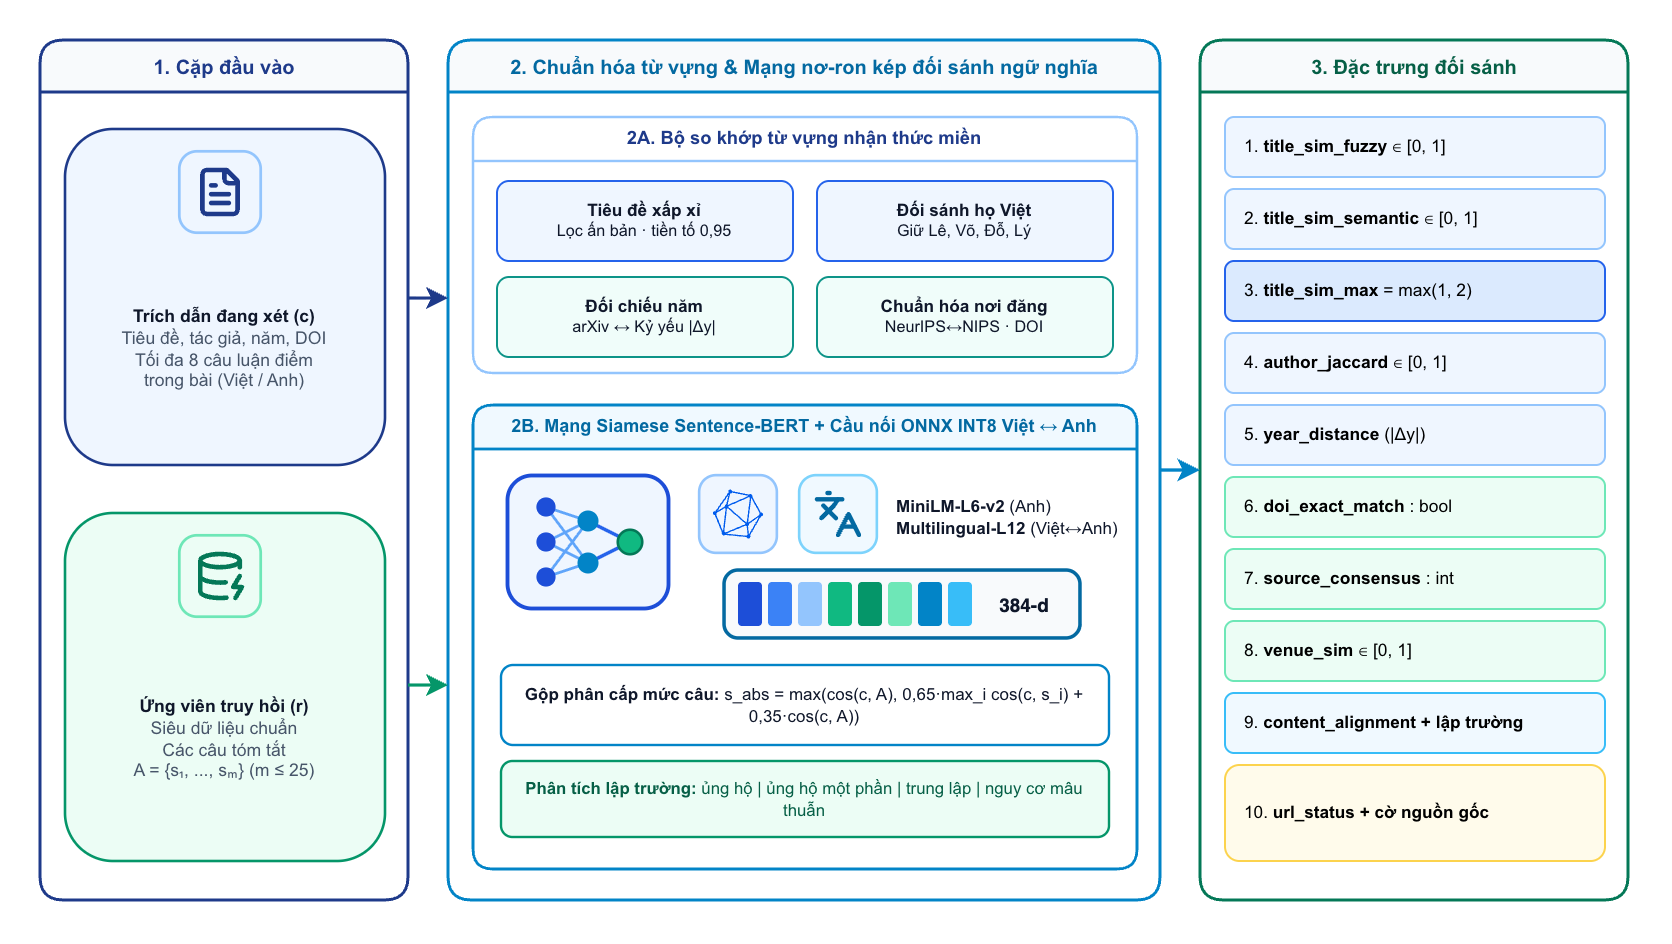
\includegraphics[width=\textwidth,keepaspectratio]{picture/figures/fig4_5_matching.png}
    \caption[Kiến trúc đối sánh từ vựng, ngữ nghĩa và xuyên ngôn ngữ bộ mã hóa kép]{Kiến trúc tầng đối sánh kết hợp chuẩn hóa từ vựng, căn chỉnh tóm tắt gộp theo câu bằng Sentence-BERT ($0.65\,\max + 0.35\,\mathrm{abs}$), cổng lập trường và bắc cầu \texttt{VI}$\leftrightarrow$\texttt{EN} ONNX INT8.}
    \label{fig:matching}
\end{figure}

\section{Kiểm chứng lai Nơ-ron -- Ký hiệu và hiệu chỉnh xác suất Platt}

\subsection{Cây quyết định ký hiệu phân cấp ưu tiên}

\texttt{NeuroSymbolicChecker} dung hợp các đặc trưng căn chỉnh nơ-ron với cây quyết định ký hiệu tất định gồm \textbf{68 mã luật \texttt{R-*} thực thi phân biệt}---65 mã tĩnh (57 mã định nghĩa trong \texttt{logic/rules.py} cùng 8 mã trong \texttt{neuro\_symbolic\_checker.py} và \texttt{vn\_legal\_verifier.py}, được tiêu thụ bởi \texttt{cis.py}) cộng 3 mã điều chỉnh nguồn gốc gắn tiền tố động (\texttt{R-LOCAL\_DB}, \texttt{R-API\_EXHAUSTED}, \texttt{R-LOCAL\_DB\_ONLY} tạo qua \texttt{f"R-\{warning\}"} trong \texttt{rules.py}; tổng hợp hệ phân loại tại Phụ lục~\ref{app:taxonomy})---kết hợp mô hình Hồi quy Logistic Đa lớp 16 đặc trưng và bộ hiệu chỉnh Platt, thể hiện ở Hình~\ref{fig:neurosymbolic} và Bảng~\ref{tab:rules}. Để tối ưu độ trễ, nhánh nhanh \texttt{is\_known\_paper()} kiểm chứng 101 công trình kinh điển trong \texttt{\_KNOWN\_PAPERS} trước khi pha trộn tổng quát nhưng vẫn kiểm tra chặt năm xuất bản, tác giả và lập trường; các trích dẫn học thuật thông thường đi qua tiền sàng lọc Bậc~0 và 16 nhóm luật như tóm lược trong sơ đồ luồng quyết định có rào chắn ở Hình~\ref{fig:decision-flow}.

\begin{figure}[!htbp]
    \centering
    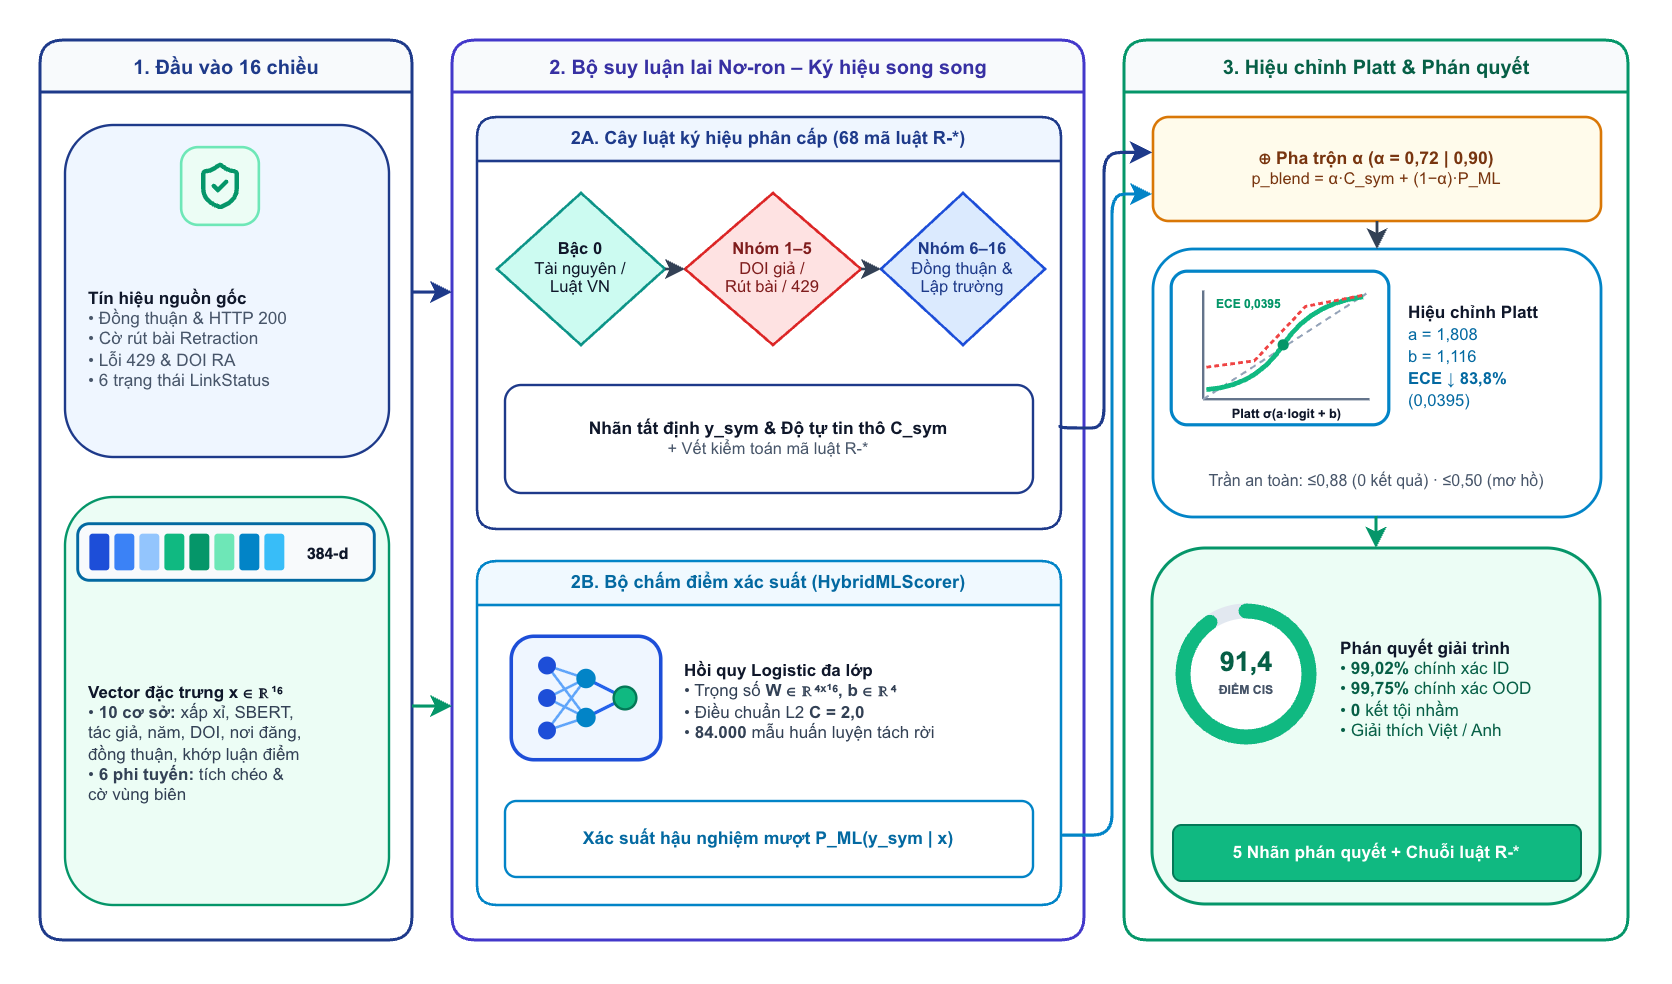
\includegraphics[width=\textwidth,keepaspectratio]{picture/figures/fig4_6_neurosymbolic.png}
    \caption[Bộ kiểm chứng lai Nơ-ron -- Ký hiệu và hiệu chỉnh xác suất Platt]{Kiến trúc kiểm chứng lai Nơ-ron -- Ký hiệu dung hợp bộ suy diễn 16 nhóm luật ký hiệu (68 mã \texttt{R-*}) với mô hình Hồi quy Logistic Đa lớp 16 đặc trưng và hiệu chỉnh xác suất Platt trên không gian logit.}
    \label{fig:neurosymbolic}
\end{figure}

{\setlength{\tabcolsep}{3.5pt}
\begin{longtable}{|C{0.11}|L{0.33}|L{0.56}|}
\caption{Thứ tự đánh giá của tiền sàng lọc ký hiệu và 16 nhóm luật kiểm chứng (68 mã \texttt{R-*}).}\label{tab:rules}\\
\hline
\textbf{Nhóm} & \textbf{Mã luật đại diện} & \textbf{Điều kiện kích hoạt và Nhãn phán quyết} \\
\hline
\endfirsthead
\multicolumn{3}{c}{\itshape Bảng \thetable\ (tiếp theo trang trước)}\\
\hline
\textbf{Nhóm} & \textbf{Mã luật đại diện} & \textbf{Điều kiện kích hoạt và Nhãn phán quyết} \\
\hline
\endhead
\hline
\multicolumn{3}{r}{\itshape Xem tiếp trang sau}\\
\endfoot
\hline
\endlastfoot
\textbf{Bậc 0} & \texttt{R-URL-RESOURCE}, \texttt{R-WEB-RESOURCE}, \texttt{R-VN-LEGAL-VERIFIED}, \texttt{R-VN-LEGAL-\allowbreak MISMATCH} & Tài liệu web thuần túy, thành phần phần mềm/RFC/HF hoặc văn bản pháp luật Việt Nam kiểm tra qua \texttt{VNLegalVerifier} $\rightarrow$ \textbf{\texttt{resource}} (hoặc \texttt{metadata\_error}/\texttt{suspected\_hallucination} nếu sai thẩm quyền/số hiệu). \\
\hline
\textbf{1} & \texttt{R-FAKE-URL}, \texttt{R-FABRICATED-DOI}, \texttt{R-CHIMERIC-DOI-\allowbreak MISMATCH}, \texttt{R-RETRACTED-PAPER} & Tên miền giả RFC 2606, tiền tố DOI chưa đăng ký hoặc DOI thật phân giải ra tiêu đề không liên quan $\rightarrow$ \textbf{\texttt{suspected\_hallucination}}; cờ rút bài Retraction Watch (\texttt{is\_retracted}) $\rightarrow$ \textbf{\texttt{metadata\_error}}. \\
\hline
\textbf{2} & \texttt{R-FUTURE-YEAR}, \texttt{R-FUTURE-YEAR-\allowbreak{}KNOWN-AUTHOR} & Năm trích dẫn vượt năm hiện tại $+ 1$: công trình lạ $\rightarrow$ \textbf{\texttt{suspected\_hallucination}}; công trình/tác giả có thật $\rightarrow$ \textbf{\texttt{metadata\_error}}. \\
\hline
\textbf{3} & \texttt{R-KNOWN-PAPER}, \texttt{R-TITLE-MISMATCH} & Khớp danh sách 101 công trình kinh điển: đồng nhất siêu dữ liệu và lập trường $\rightarrow$ \textbf{\texttt{verified}}; sai năm/tác giả/nhận định $\rightarrow$ \textbf{\texttt{metadata\_error}}. \\
\hline
\textbf{4} & \texttt{R-DEAD-URL}, \texttt{R-NONEXISTENT-DOI}, \texttt{R-NO-SCHOLARLY-\allowbreak RECORD} & Không có ứng viên khi $\ge 2$ API trực tuyến trả HTTP 200 sạch (hoặc xác nhận URL chết không có bản lưu) $\rightarrow$ \textbf{\texttt{suspected\_hallucination}} (chặn trần $\le 0.88$ nếu chỉ do vắng mặt bản ghi). \\
\hline
\textbf{5} & \texttt{R-FAIL-ALL}, \texttt{R-RATE-LIMITED-\allowbreak ABSTAIN}, \texttt{R-DOI-RA-NO-CSL} & Không có ứng viên do cạn hạn mức HTTP 429, lỗi mạng hoặc DOI khu vực hợp lệ không công bố siêu dữ liệu CSL $\rightarrow$ \textbf{\texttt{unresolved}}. \\
\hline
\textbf{6} & \texttt{R-DOI-TITLE-AUTHOR} & Khớp chính xác DOI trực tuyến kèm $\texttt{title\_sim} \ge 0.90$ và $\texttt{author\_jaccard} \ge 0.50$ $\rightarrow$ \textbf{\texttt{verified}}. \\
\hline
\textbf{7} & \texttt{R-LOCAL\_DB\_VERIFIED}, \texttt{R-LOCAL\_DB\_GOOD\_MATCH} & Khớp chỉ mục FTS5 ngoại tuyến ($\texttt{title\_sim\_fuzzy} \ge 0.95$, $\texttt{author\_jaccard} \ge 0.80$, $|\Delta y| = 0$) không xung đột DOI $\rightarrow$ \textbf{\texttt{verified}}. \\
\hline
\textbf{8} & \texttt{R-WELL-LINKED}, \texttt{R-WELL-LINKED-\allowbreak MODERATE} & Trích dẫn đã liên kết (\texttt{matched}) có độ khớp cao về tiêu đề/tác giả/năm và không mâu thuẫn định danh $\rightarrow$ \textbf{\texttt{verified}}. \\
\hline
\textbf{9} & \texttt{R-DOI-TITLE-\allowbreak MISMATCH} & DOI trực tuyến phân giải thành công nhưng độ tương đồng tiêu đề nằm trong $[0.60, 0.90)$ $\rightarrow$ \textbf{\texttt{metadata\_error}} kèm trường sai lệch. \\
\hline
\textbf{10} & \texttt{R-CONSENSUS-FULL}, \texttt{R-CONSENSUS-\allowbreak PARTIAL} & Từ $\ge 2$ cơ sở dữ liệu đồng thuận tiêu đề ($\ge 0.90$) không xung đột DOI: khớp tác giả/năm $\rightarrow$ \textbf{\texttt{verified}}; lệch tác giả/năm $\rightarrow$ \textbf{\texttt{metadata\_error}}. \\
\hline
\textbf{11} & \texttt{R-SINGLE-SOURCE-\allowbreak VERIFIED}, \texttt{R-BOOK-EDITION-\allowbreak VERIFIED}, \texttt{R-SINGLE-SOURCE-\allowbreak PARTIAL} & Khớp một nguồn trực tuyến duy nhất ($\ge 0.90$ tiêu đề, $\ge 0.80$ tác giả, $|\Delta y| \le 1$, hoặc $\le 15$ năm giữa ấn bản sách OpenLibrary) $\rightarrow$ \textbf{\texttt{verified}}; sai lệch trường $\rightarrow$ \textbf{\texttt{metadata\_error}}. \\
\hline
\textbf{12} & \texttt{R-AMBIGUOUS-\allowbreak MAPPING} & Bộ liên kết hai phía gắn cờ \texttt{ambiguous\_mapping} $\rightarrow$ \textbf{\texttt{unresolved}} với trần độ tin cậy $0.50$. \\
\hline
\textbf{13} & \texttt{R-CONTENT-\allowbreak ALIGNMENT}, \texttt{R-CONTENT-MISMATCH} & Đối sánh ngữ cảnh -- tóm tắt cao cứu các tiêu đề viết tắt ($\rightarrow$ \textbf{\texttt{verified}}); nhận định trong bài mâu thuẫn công trình gốc $\rightarrow$ \textbf{\texttt{metadata\_error}}. \\
\hline
\textbf{14} & \texttt{R-KNOWN-AUTHOR-\allowbreak TITLE-MISMATCH} & Tác giả học thuật có thật đi kèm tiêu đề lệch trong $[0.30, 0.90)$ $\rightarrow$ \textbf{\texttt{metadata\_error}}. \\
\hline
\textbf{15} & \texttt{R-ABSTENTION-\allowbreak BORDER}, \texttt{R-DOMAIN-EXCEPTION} & Độ tương đồng tiêu đề ở vùng giáp ranh $[0.40, 0.60)$ $\rightarrow$ \textbf{\texttt{unresolved}}; bài báo xác thực có URL ngoài chết bật \texttt{domain\_exception = True}. \\
\hline
\textbf{16} & \texttt{R-WEAK-EVIDENCE}, \texttt{R-HALLUCINATED-\allowbreak SOURCE} & Nhánh cuối ($\texttt{title\_sim} < 0.40$): có $\ge 2$ API trực tuyến phản hồi sạch + chồng lấn tác giả thấp $\rightarrow$ \textbf{\texttt{suspected\_hallucination}}; ngược lại $\rightarrow$ \textbf{\texttt{unresolved}}. \\
\hline
\end{longtable}
}

\begin{figure}[!htbp]
    \centering
    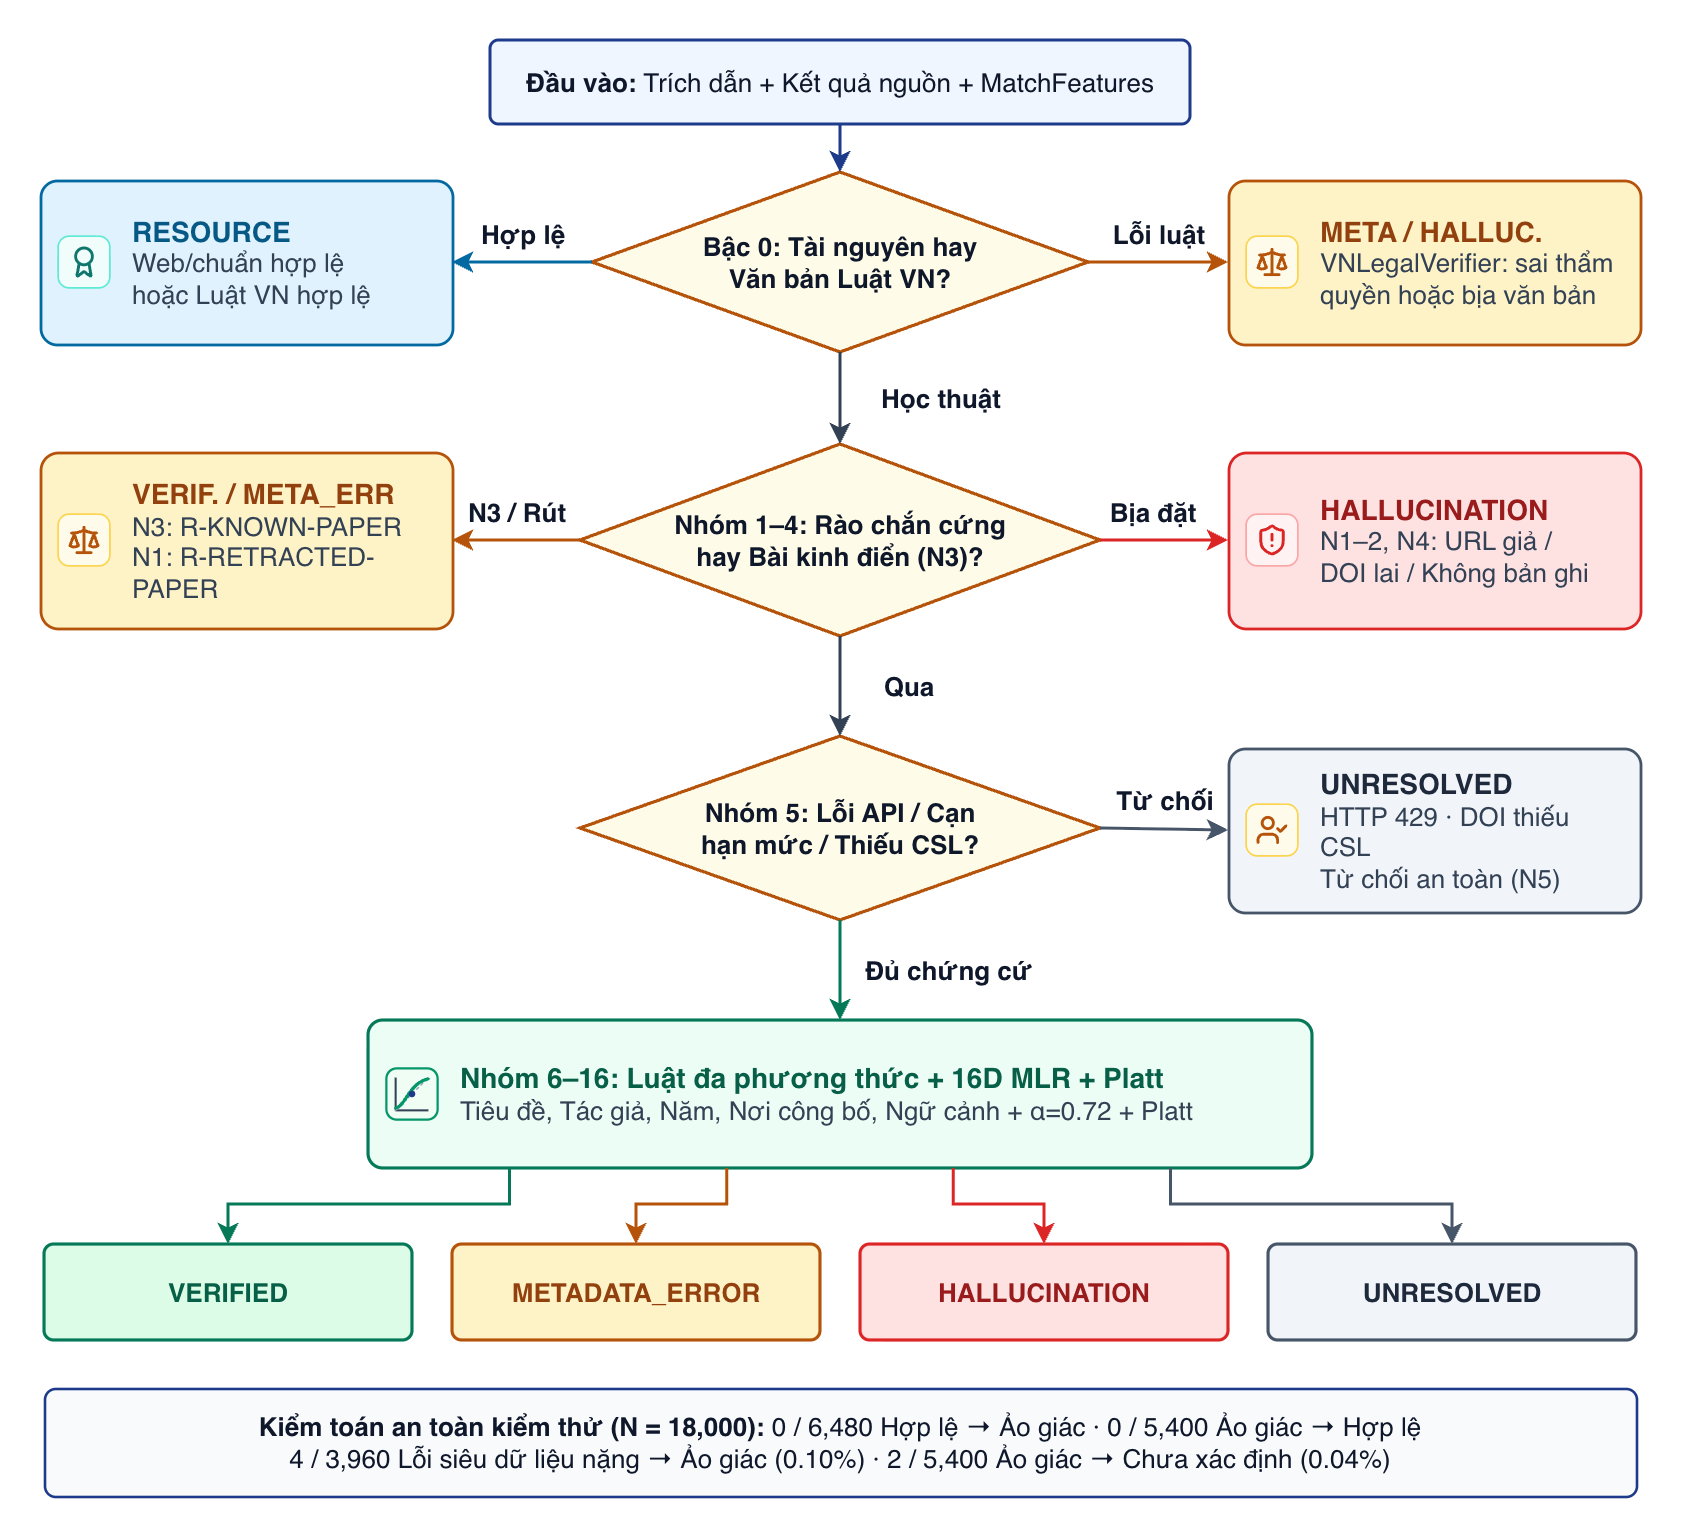
\includegraphics[width=\textwidth,keepaspectratio]{picture/figures/fig4_7_decision_flow.png}
    \caption[Luồng quyết định lai Nơ-ron -- Ký hiệu có rào chắn qua Bậc 0 và Nhóm 1--16]{Luồng quyết định lai Nơ-ron -- Ký hiệu đầu--cuối minh họa cách CITRA định tuyến trích dẫn qua tiền sàng lọc Bậc 0, rào chắn ký hiệu ưu tiên cao (Nhóm 1--5), chấm điểm bằng chứng (Nhóm 6--16) và hiệu chỉnh Platt trên không gian logit.}
    \label{fig:decision-flow}
\end{figure}

Hai cơ chế bảo vệ nguồn gốc ngăn ngừa cáo buộc sai quá tự tin: Nhóm 4 (\texttt{R-NO-SCHOLARLY-RECORD}) chỉ kích hoạt khi có ít nhất hai API trực tuyến trả mã HTTP 200 rỗng hợp lệ (ngược lại Nhóm 5 buộc trả \texttt{unresolved}), và mọi nghi vấn ảo giác chỉ dựa trên sự vắng mặt bản ghi luôn bị chặn trần độ tin cậy sau hiệu chỉnh ở mức $\le 0.88$.

\subsection{Hồi quy Logistic 16 đặc trưng, thuật toán hình thức và hiệu chỉnh Platt}

Để chuyển đổi kết quả ký hiệu rời rạc thành xác suất hiệu chỉnh mượt, \texttt{HybridMLScorer.extract\_feature\_vector()} tạo véc-tơ $\mathbf{x} \in \mathbb{R}^{16}$ gồm mười tín hiệu cơ sở ($x_1 = t_{\text{fuzz}}$, $x_2 = t_{\text{sem}}$, $x_3 = t_{\max} = \max(t_{\text{fuzz}}, t_{\text{sem}})$, $x_4 = a_J$ [\texttt{author\_jaccard}], $x_5 = y_m = 0$ nếu $|\Delta y| \ge 50$ ngược lại $\exp(-0.5\min(|\Delta y|, 10))$, $x_6 = d_{\text{ok}} \in \{0, 1\}$, $x_7 = \min(\text{consensus}, 4)/4$, $x_8 = v_{\text{sim}}$, $x_9 = s_{\text{content}}$ nếu $(\text{thẳng hàng} \land s_{\text{content}} \ge 0.45 \land \neg\texttt{contradiction\_risk})$, $-0.6$ nếu $(\neg\text{thẳng hàng} \land (\texttt{contradiction\_risk} \lor 0 < s_{\text{content}} < 0.46))$, ngược lại $0$, $x_{10} = h_{\text{cand}} \in \{0, 1\}$) và sáu đặc trưng tương tác tại Phương trình~\eqref{eq:ml-interactions}:
\begin{equation}\label{eq:ml-interactions}
\begin{aligned}
x_{11} &= t_{\max}\, a_J, & x_{12} &= t_{\max}\, y_m, \\
x_{13} &= t_{\max}(1 - a_J)\,\mathbb{I}[t_{\max} \ge 0.60], & x_{14} &= t_{\max}(1 - y_m)\,\mathbb{I}[t_{\max} \ge 0.60], \\
x_{15} &= d_{\text{ok}}(1 - t_{\max}), & x_{16} &= \mathbb{I}[\text{vùng từ chối phán quyết}],
\end{aligned}
\end{equation}
trong đó $x_{16} = 1$ khi (i)~$h_{\text{cand}} = 0$ kèm cạn hạn mức API hoặc \texttt{registered\_no\_csl}, hoặc (ii)~$d_{\text{ok}} = 0 \land h_{\text{cand}} = 1$ rơi vào dải tiêu đề giáp ranh ($0.40 \le t_{\max} < 0.60$ có tín hiệu tác giả/từ vựng/đồng thuận) hay dải xám tác giả bán phần ($0.25 \le t_{\max} < 0.60 \land a_J \ge 0.18 \land |\Delta y| \le 3$).

\begin{citraalgo}{4.2}{\texttt{NeuroSymbolicVerifyAndCalibrate}$(r, \mathcal{S}, \mathbf{f}, \delta_{\text{style}})$}{alg:verify}
\textbf{Đầu vào:} Mục tham khảo $r$, kết quả truy hồi $\mathcal{S}$, đặc trưng đối sánh $\mathbf{f}$, mức phạt phong cách $\delta_{\text{style}} \in [0, 0.15]$.\\
\textbf{Đầu ra:} Phán quyết cuối $(y^*, P_{\text{cal}}, \mathcal{R}_{\text{rules}})$.
{\setlength{\leftmargini}{1.6em}
\begin{enumerate}\setlength{\itemsep}{1pt}\setlength{\parskip}{0pt}
\item \textbf{Bậc 0:} Nếu $r$ là tài nguyên web/phần mềm/RFC hoặc văn bản pháp luật VN (\texttt{VNLegalVerifier}), kiểm tra URL giả/chết trước; trả về \texttt{resource} (hoặc \texttt{metadata\_error}/\texttt{suspected\_hallucination}) tương ứng.
\item \textbf{Nhánh nhanh công trình kinh điển:} Nếu $r$ khớp \texttt{\_KNOWN\_PAPERS} (101 bài báo), kiểm tra năm/tác giả/lập trường và trả về \texttt{verified} hoặc \texttt{metadata\_error} kèm \texttt{R-KNOWN-PAPER}.
\item \textbf{Cây ký hiệu:} Đánh giá Nhóm 1--16 trong \texttt{SymbolicRules.apply}$(r, \mathcal{S}, \mathbf{f}, \delta_{\text{style}})$ $\rightarrow (y_{\text{sym}}, C_{\text{sym}}, \mathcal{R}_{\text{rules}})$, áp dụng cảnh báo nguồn gốc (\texttt{LOCAL\_DB}: $-0.05$, \texttt{API\_EXHAUSTED}: $-0.10$, \texttt{LOCAL\_DB\_ONLY}: $-0.15$, xuất với tiền tố \texttt{R-}) và $\delta_{\text{style}}$.
\item \textbf{Chấm điểm học máy:} Trích xuất $\mathbf{x} \in \mathbb{R}^{16}$ (Phương trình~\eqref{eq:ml-interactions}) và tính $P_{\text{ML}}(y \mid \mathbf{x}) = \operatorname{softmax}(W\mathbf{x} + \mathbf{b})_y$.
\item \textbf{Pha trộn thích ứng:} Nếu $C_{\text{sym}} \le 0$, trả ngay $P_{\text{cal}} \leftarrow 0.0$; ngược lại khôi phục $C_{\text{base}} = \min(0.99, C_{\text{sym}} + \delta_{\text{style}})$, đặt $\alpha \leftarrow 0.90$ nếu $C_{\text{base}} \ge 0.85 \land |C_{\text{base}} - P_{\text{ML}}(y_{\text{sym}} \mid \mathbf{x})| > 0.45$ còn lại $0.72$, và tính $p_{\text{blend}} = \alpha C_{\text{base}} + (1 - \alpha) P_{\text{ML}}(y_{\text{sym}} \mid \mathbf{x})$.
\item \textbf{Hiệu chỉnh Platt \& Tái áp dụng phạt phong cách:} Tính $P_{\text{cal}}$ theo Phương trình~\eqref{eq:platt-calib} với $(a_{\text{cal}}, b_{\text{cal}}) = (1.891263, 1.138599)$; nếu $\delta_{\text{style}} > 0$, đặt $P_{\text{cal}} \leftarrow \max(0.05, P_{\text{cal}} - \delta_{\text{style}})$.
\item \textbf{Rào chắn hậu hiệu chỉnh:} Chặn $P_{\text{cal}} \le 0.50$ nếu kích hoạt \texttt{R-AMBIGUOUS-MAPPING}; chặn $P_{\text{cal}} \le \max(0.05, 0.88 - \delta_{\text{style}})$ nếu $y_{\text{sym}} = \texttt{suspected\_hallucination}$ chỉ dựa trên vắng mặt bản ghi; gán $y^* \leftarrow y_{\text{sym}}$ (áp dụng \texttt{\_apply\_dead\_link\_exception()} nếu bài bị rút lại hoặc có URL chết); \textbf{trả về} $(y^*, P_{\text{cal}}, \mathcal{R}_{\text{rules}})$.
\end{enumerate}}
\end{citraalgo}

Thuật toán~\ref{alg:verify} hình thức hóa toàn bộ luồng suy diễn và hiệu chỉnh trong \texttt{NeuroSymbolicChecker}. Mô hình Hồi quy Logistic Đa lớp ($W \in \mathbb{R}^{4 \times 16}, \mathbf{b} \in \mathbb{R}^4$, $C = 0.25$, trọng số lớp cân bằng trên 84,000 mẫu huấn luyện phân tách theo bài báo) bảo toàn quyền ưu tiên của luật ký hiệu đồng thời cung cấp mật độ xác suất liên tục; do $b_{\text{cal}} = +1.138599$ phản ánh độ chính xác tổng thể cao ($99.67\%$), các điểm \texttt{unresolved} quanh $p_{\text{blend}} = 0.50$ được hiệu chỉnh lên $0.7574$ (biểu thị mức tin cậy cao vào \emph{quyết định từ chối phán quyết}), trong khi \texttt{R-AMBIGUOUS-MAPPING} chủ động ghim trần ở $0.50$.

\section{Chấm điểm toàn vẹn và giải thích song ngữ}

\subsection{Điểm toàn vẹn trích dẫn (CIS) năm thành phần}

Phương thức \texttt{CISCalculator.compute()} tổng hợp bằng chứng toàn bản thảo vào đoạn $[0, 100]$. Danh mục rỗng ($N = 0$) trả về $\text{CIS} = 0.00$. Các mục \texttt{resource} phi học thuật được loại khỏi mẫu số học thuật $N_{\text{acad}}$ để tài liệu kỹ thuật hoặc văn bản pháp luật không làm méo tỷ lệ xác thực khoa học. Trong trường hợp biên danh mục chỉ gồm tài nguyên web/pháp lý ($N \ge 1, N_{\text{acad}} = 0$), hệ thống tính $s_{\text{id}}$ trên mọi URL/DOI tài nguyên, và khi $N \ge 3$ có thông tin liên kết sẽ nhân điều chỉnh $s_{\text{ver}} = s_{\text{meta}} = (0.5 + 0.5\,\rho_{\text{cited}})\,s_{\text{id}}$ để các danh mục web không được trích dẫn trong bài không đạt điểm ảo.

Với bản thảo có $N_{\text{acad}} \ge 1$, năm thành phần tại Bảng~\ref{tab:cis} được định nghĩa đầy đủ bởi Phương trình~\eqref{eq:cis-ver}--\eqref{eq:cis-total}:
\begin{align}
s_{\text{ver}} &= \frac{N_{\text{verified}}}{N_{\text{acad}}}, \label{eq:cis-ver}\\
s_{\text{meta}} &= \max\!\left(0,\; 1 - \frac{0.50\,N_{\text{meta\_std}} + 0.75\,N_{\text{meta\_incomp}} + 1.00\,N_{\text{hall}}}{N_{\text{acad}}}\right), \label{eq:cis-meta}\\
s_{\text{link}} &= \max\!\left(0,\; 1 - \frac{\sum_{e \in \mathcal{L}} \pi(e) + 0.10\,N_{\text{uncited}} + 0.10\,N_{\text{dup}}}{|\mathcal{L}| + N_{\text{uncited}} + N_{\text{dup}}}\right), \label{eq:cis-link}\\
\text{CIS} &= 100 \times \bigl(0.35\,s_{\text{ver}} + 0.25\,s_{\text{meta}} + 0.25\,s_{\text{link}} + 0.10\,s_{\text{fmt}} + 0.05\,s_{\text{id}}\bigr), \label{eq:cis-total}
\end{align}
trong đó $s_{\text{link}}$ bị chặn trần $\le 0.50$ khi $100\%$ mục tài liệu không được trích dẫn và không có liên kết nội văn nào khớp; $s_{\text{fmt}}$ ánh xạ từ độ tin cậy \texttt{StyleProfile} ($0.8 + 0.2\,\text{conf}$ khi đồng nhất chuẩn nhận diện, $0.5$ khi \texttt{UNKNOWN}, hằng số $0.4$ khi \texttt{MIXED}, giảm $0.2$ và chặn sàn $0.2$ nếu bật cờ \texttt{style\_inconsistent}, chỉ dùng dự phòng từng mục $\max(0.3, 1 - N_{\text{incons}} / N)$ hoặc $0.8$ khi thiếu \texttt{StyleProfile}); còn $s_{\text{id}} = N_{\text{valid\_id}} / N_{\text{with\_id}}$ chỉ tính định danh hợp lệ khi không dính luật định danh sai, \texttt{domain\_exception}, \texttt{dead\_link} hay \texttt{fake\_domain} \emph{và} nhãn kết luận là \texttt{verified} hoặc \texttt{metadata\_error} (mặc định $1.00$ khi $N_{\text{with\_id}} = 0$ để không phạt oan các chuẩn nhân văn không ghi DOI).

Bộ trọng số mặc định phân bổ $60\%$ cho tính xác thực nguồn ($0.35\,s_{\text{ver}} + 0.25\,s_{\text{meta}}$), $25\%$ cho kỷ luật liên kết cấu trúc ($s_{\text{link}}$) và $15\%$ cho định dạng cùng định danh ($0.10\,s_{\text{fmt}} + 0.05\,s_{\text{id}}$), đạt độ ổn định thứ hạng Spearman $\rho = 0.9987$ khi nhiễu loạn trọng số (Chương~\ref{chap:results}). Hai đặc tính biên được làm rõ cho giảng viên: (i)~việc không ghi DOI/URL cho $s_{\text{id}} = 1.00$ để tránh phạt bất công nguồn sách in; và (ii)~mục \texttt{unresolved} không nhận điểm ở $s_{\text{ver}}$ (mất tối đa $35$ điểm) nhưng không bị phạt siêu dữ liệu ở $s_{\text{meta}}$ nhằm bảo toàn nguyên tắc suy đoán vô tội. Vì vậy, \textbf{CITRA} luôn hiển thị số lượng \texttt{num\_unresolved} cùng bảng tách năm thành phần cạnh vòng điểm CIS để giảng viên rà soát mọi bài có nhiều mục chưa xác định thay vì chỉ nhìn một con số tổng.

{\setlength{\tabcolsep}{3.5pt}
\begin{table}[!htbp]
\centering
\caption{Các thành phần và trọng số mặc định của Điểm toàn vẹn trích dẫn (CIS).}\label{tab:cis}
\begin{tabular}{|L{0.31}|C{0.11}|L{0.58}|}
\hline
\textbf{Thành phần} & \textbf{Trọng số} & \textbf{Định nghĩa chính xác trong \texttt{CISCalculator.compute()}} \\
\hline
\textbf{\texttt{verified\_ratio}} ($s_{\text{ver}}$) & \textbf{0.35} & $N_{\text{verified}} / N_{\text{acad}}$, tỷ lệ tài liệu tham khảo học thuật được xác thực. \\
\hline
\textbf{\texttt{metadata\_accuracy}} ($s_{\text{meta}}$) & \textbf{0.25} & Điểm trung thực siêu dữ liệu phân bậc tại Phương trình~\eqref{eq:cis-meta}. \\
\hline
\textbf{\texttt{in\_text\_bib\_consistency}} ($s_{\text{link}}$) & \textbf{0.25} & Độ nhất quán liên kết hai phía (Phương trình~\eqref{eq:cis-link}, chặn $\le 0.50$ nếu 0\% trích dẫn). \\
\hline
\textbf{\texttt{format\_consistency}} ($s_{\text{fmt}}$) & \textbf{0.10} & Độ nhất quán chuẩn trình bày từ \texttt{StyleProfile} ($0.8 + 0.2\,\text{conf}$ đồng nhất, $0.5$ \texttt{UNKNOWN}, $0.4$ \texttt{MIXED}, $-0.2$ nếu lệch chuẩn; dự phòng từng mục khi thiếu). \\
\hline
\textbf{\texttt{identifier\_validity}} ($s_{\text{id}}$) & \textbf{0.05} & Tỷ lệ trích dẫn có DOI/URL đạt nhãn \texttt{verified}/\texttt{metadata\_error} và không dính luật định danh sai, \texttt{dead\_link}, \texttt{fake\_domain} hay \texttt{domain\_exception} ($1.00$ nếu không có). \\
\hline
\end{tabular}
\end{table}
}

\subsection{Giải thích phán quyết song ngữ và chuẩn hóa danh mục tham khảo}

Mọi phán quyết đi kèm lời giải thích song ngữ Anh -- Việt tất định (\texttt{logic/explanation.py} và \texttt{verdictExplanation.ts}) nêu rõ nguồn đối chứng, sai lệch từng trường, điểm ngữ nghĩa và mã luật kích hoạt. Với các mục \texttt{metadata\_error} hoặc \texttt{verified}, \texttt{bibliography\_formatter.py} và \texttt{docx\_exporter.py} tái tạo mục sạch chuẩn APA 7th, IEEE, TDTU, BibTeX và RIS từ siêu dữ liệu chính thống và xuất tệp \texttt{.docx} đã sửa lỗi trong khi cô lập mục \texttt{suspected\_hallucination} để tác giả tự loại bỏ.

\section{Tầng giao diện web (CITRA)}

\subsection{Kiến trúc frontend và cơ chế hiển thị theo cấp độ}

Ứng dụng khách nền web (\textbf{CITRA}) xây dựng bằng React 18.3, TypeScript 5.9 (dải \texttt{\string^5.4.0}, khóa phiên bản \texttt{3.90.11}), Vite, TanStack React Query và Tailwind CSS v3.4. Hai giao diện Sáng (\texttt{\#FBFAF6}) và Tối (\texttt{\#141310}) đạt chuẩn tương phản WCAG 2.1 AA và hiển thị chuẩn dấu thanh tiếng Việt. Để phục vụ cả sinh viên lẫn kiểm định viên kỹ thuật, giao diện áp dụng \emph{hiển thị theo cấp độ}: các thẻ báo cáo chính trình bày kết luận dễ hiểu trên bốn thẻ phân tích chính (\textit{Tổng quan}, \textit{Kiểm tra tài liệu tham khảo}, \textit{Kiểm tra tính nhất quán} và \textit{Xem trước tài liệu}), trong khi mã luật \texttt{R-*}, véc-tơ 16 chiều và vết thực thi 5 giai đoạn mở rộng theo yêu cầu qua khung mở rộng chi tiết có thuộc tính trợ năng \texttt{aria-expanded}. Trong quá trình tiếp nhận tệp dài, \texttt{DocumentParser.parse()} phát tiến độ đơn điệu song ngữ \texttt{[01/08]} qua \texttt{ProgressTracker} (lưu vào SQLite cho tiến trình \texttt{web\_only}), còn cơ chế bàn giao \texttt{pendingHandoffEssayId} trong \texttt{VerificationProgressContext} triệt tiêu kết nối SSE bị ngắt sớm (\texttt{HTTP 499}) khi chuyển trang. Tách gói Rollup giữ gói khởi động ở mức \textbf{$231.50\text{\,kB}$} ($67.50\text{\,kB}$ nén gzip) trên 60 gói tải trễ (gói định tuyến lớn nhất \texttt{EssayPage} đạt $250.58\text{\,kB}$ thô / $68.67\text{\,kB}$ nén gzip).

\subsection{Không gian làm việc phân quyền và bề mặt giám sát}

Các Hình~\ref{fig:ui-landing}--\ref{fig:ui-portals} giới thiệu giao diện thực tế phiên bản \texttt{v3.90.11} bản địa hóa tiếng Việt, hiển thị toàn chiều rộng trang in sau khi cắt bỏ thanh điều hướng trái để tối đa hóa độ rõ nét. Hình~\ref{fig:ui-landing} minh họa trang chủ công khai chế độ Sáng (có nút chuyển nhanh sang chế độ Tối WCAG AA trên thanh đầu trang). Hình~\ref{fig:ui-workspace} trình bày bảng điều khiển Sinh viên (hiển thị thang điểm CIS \texttt{/100}) và hàng đợi tải lên hàng loạt đa định dạng (\texttt{.pdf}, \texttt{.docx}, \texttt{.bib}, \texttt{.ris}). Hình~\ref{fig:ui-portals} thể hiện không gian phân tích lớp học của Giảng viên (số bài nộp nhất quán và bảng luật chỉ lọc các lỗi thực sự) cùng bảng Giám sát Hệ thống của Quản trị viên hiển thị kho cục bộ 129,137 bản ghi, trạng thái GROBID và các hàng độ trễ/bộ ngắt mạch trực tiếp của những nhà cung cấp tiêu biểu trong số 15 nguồn API đang hoạt động.

\begin{figure}[!htbp]
    \centering
    \fboxsep=0pt\fboxrule=0.4pt\fbox{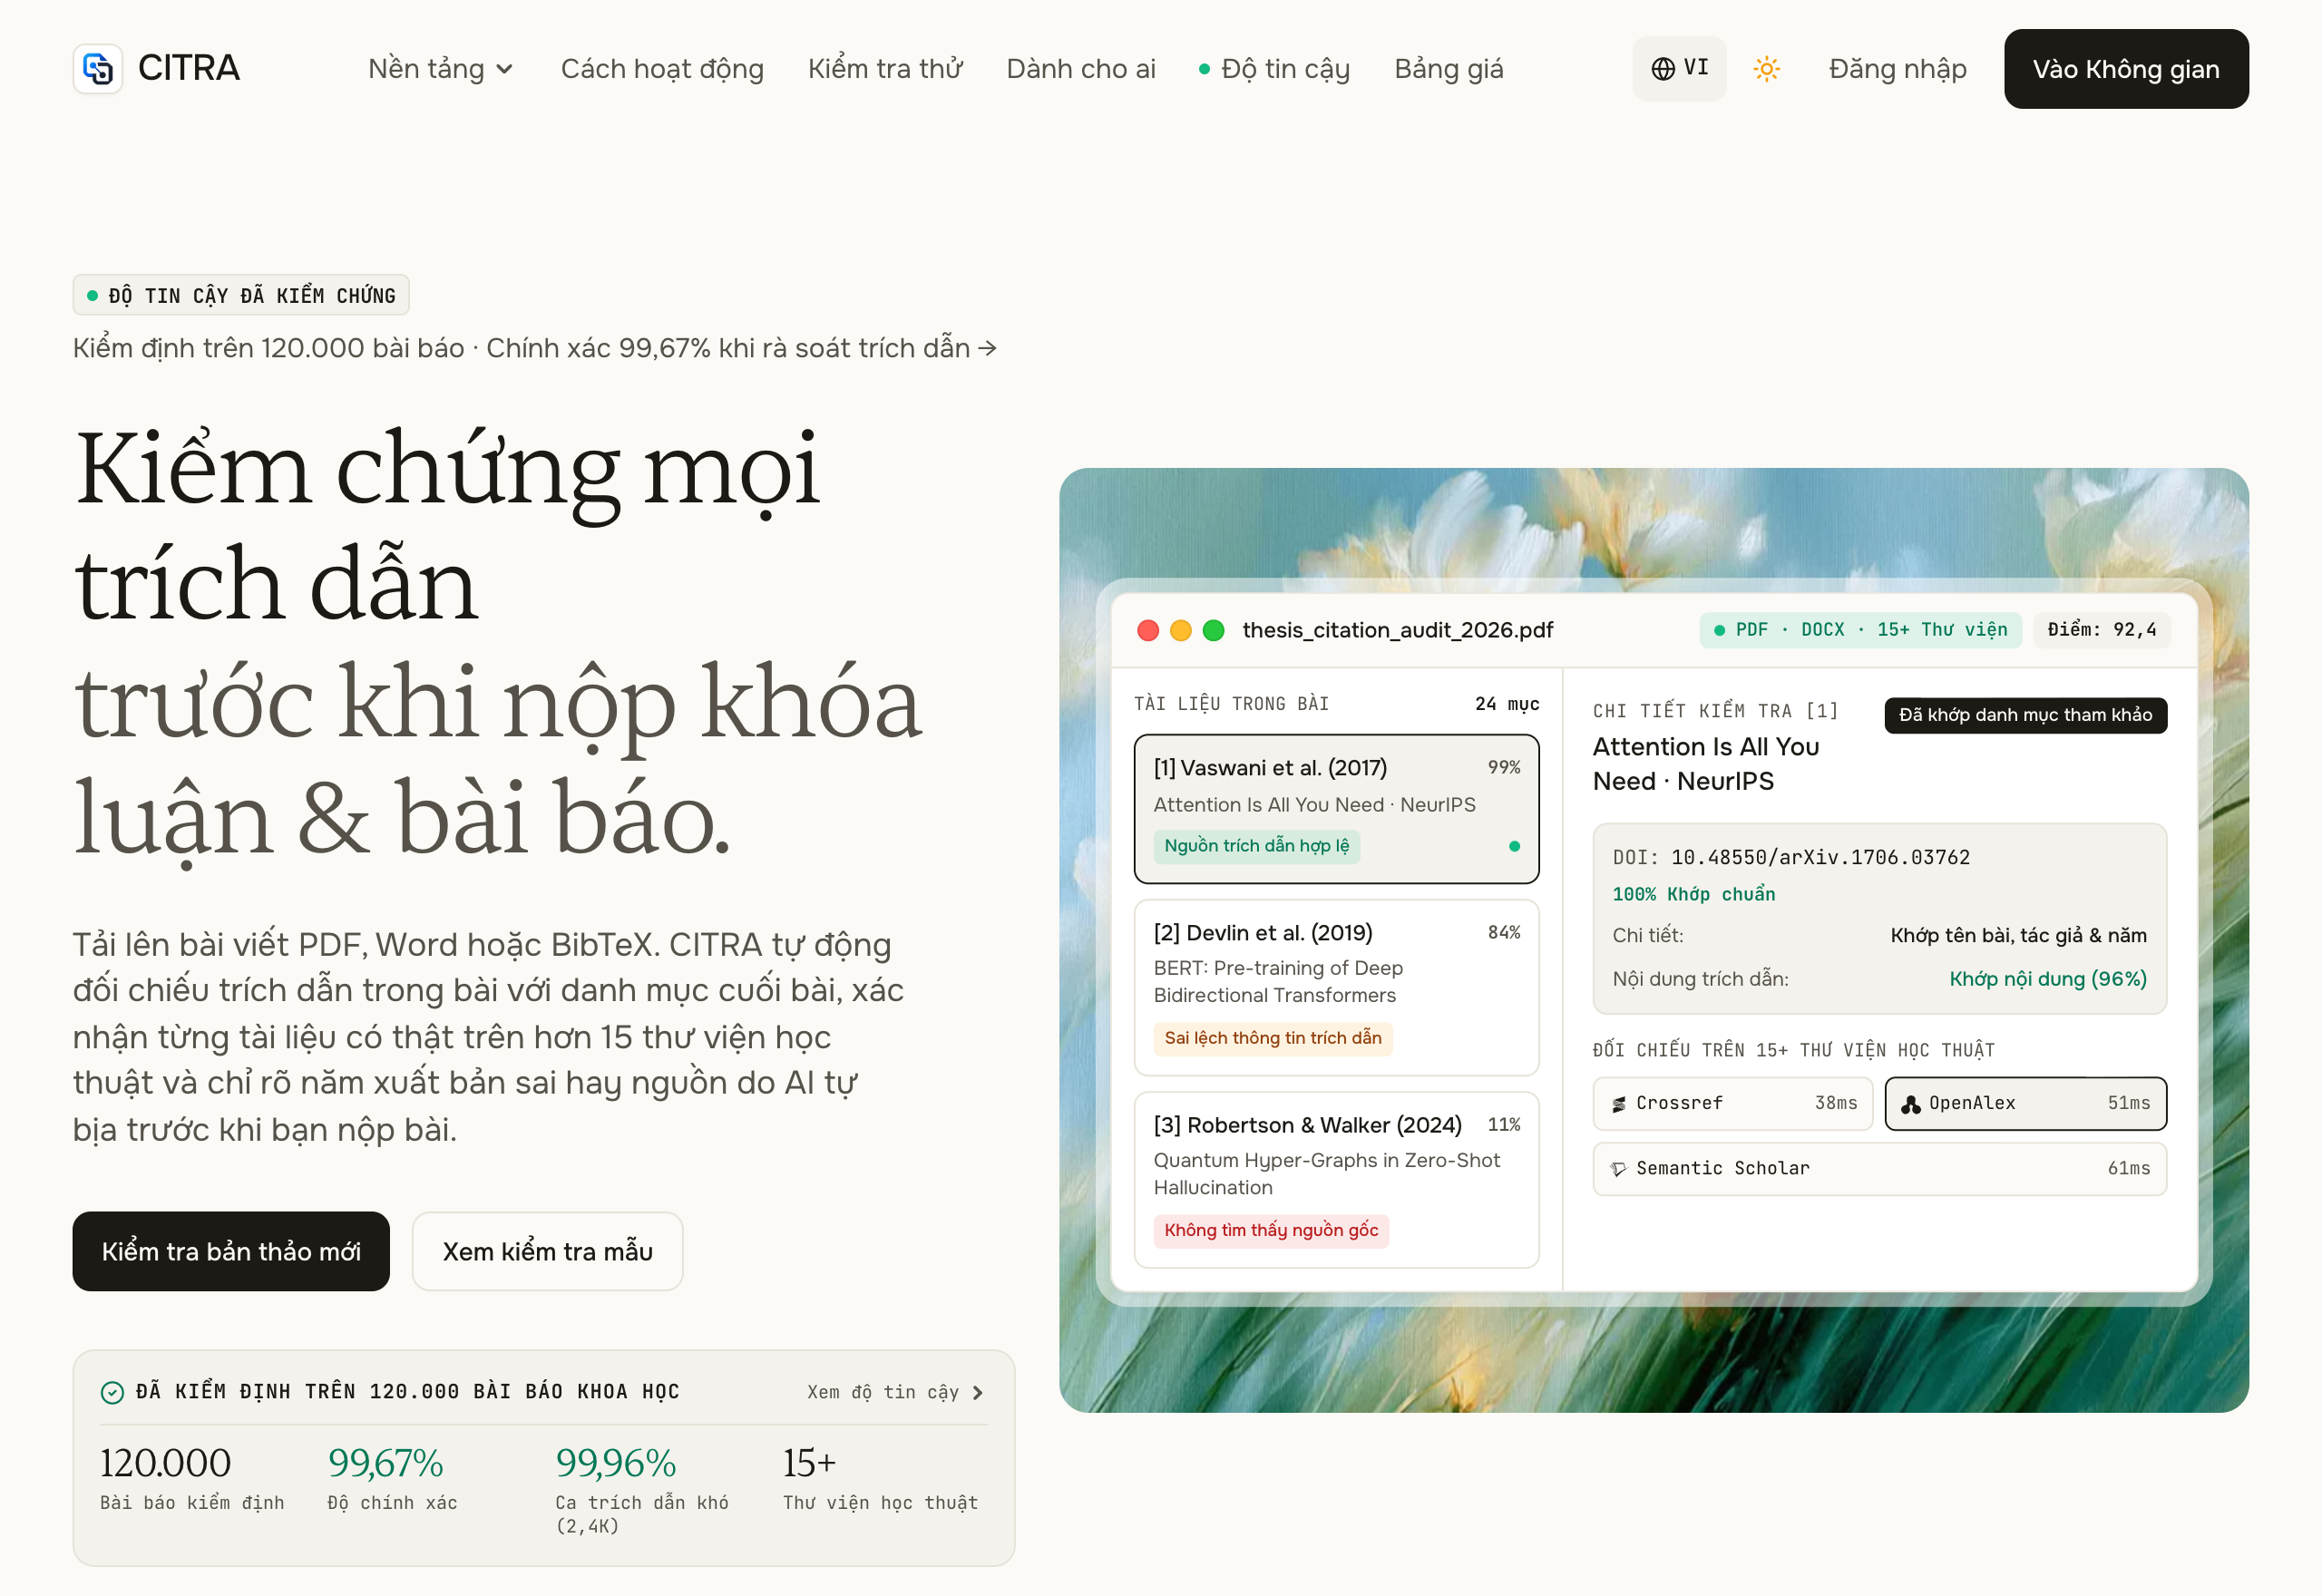
\includegraphics[width=0.96\textwidth,keepaspectratio]{picture/figures/01-landing-light.png}}
    \caption[Trang chủ CITRA chế độ Sáng đạt chuẩn tương phản WCAG AA]{Trang chủ công khai CITRA (\texttt{v3.90.11}) ở chế độ Sáng chuẩn WCAG 2.1 AA (hỗ trợ chuyển sang chế độ Tối trên thanh đầu trang).}
    \label{fig:ui-landing}
\end{figure}

\begin{figure}[!htbp]
    \centering
    \fboxsep=0pt\fboxrule=0.4pt\fbox{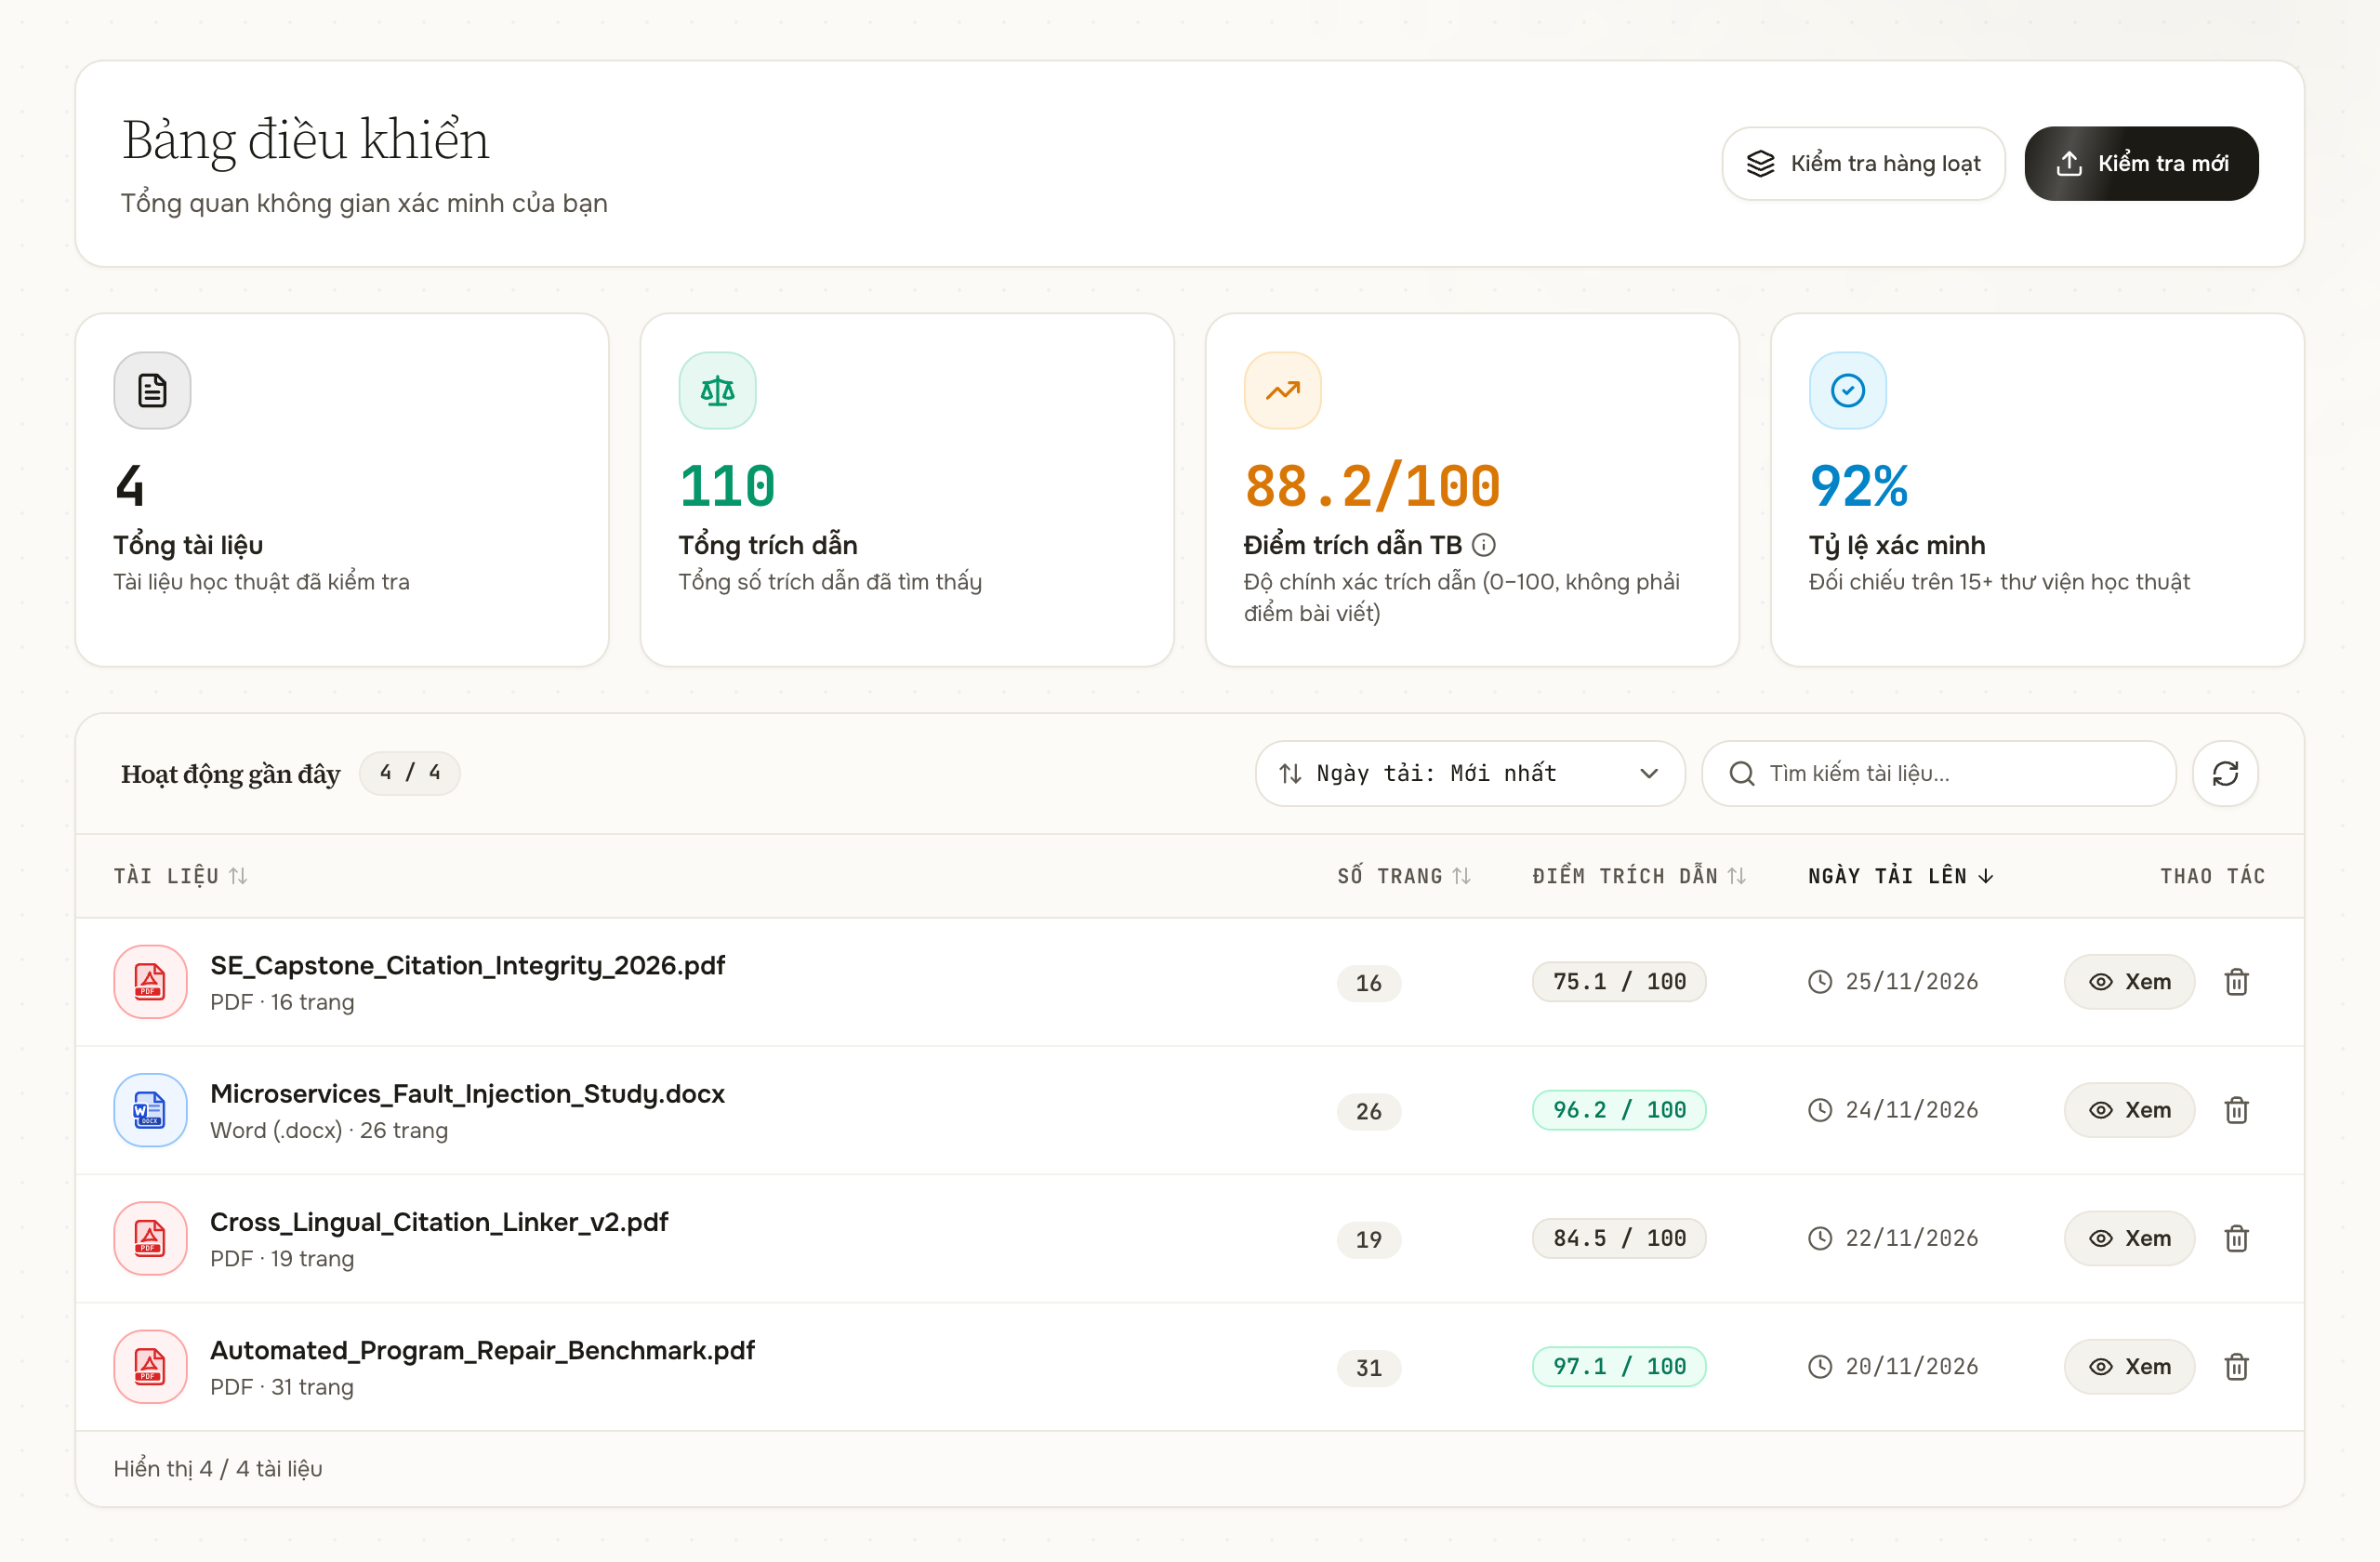
\includegraphics[width=0.94\textwidth,height=0.40\textheight,keepaspectratio]{picture/figures/03-dashboard-light.png}}\\[6pt]
    \fboxsep=0pt\fboxrule=0.4pt\fbox{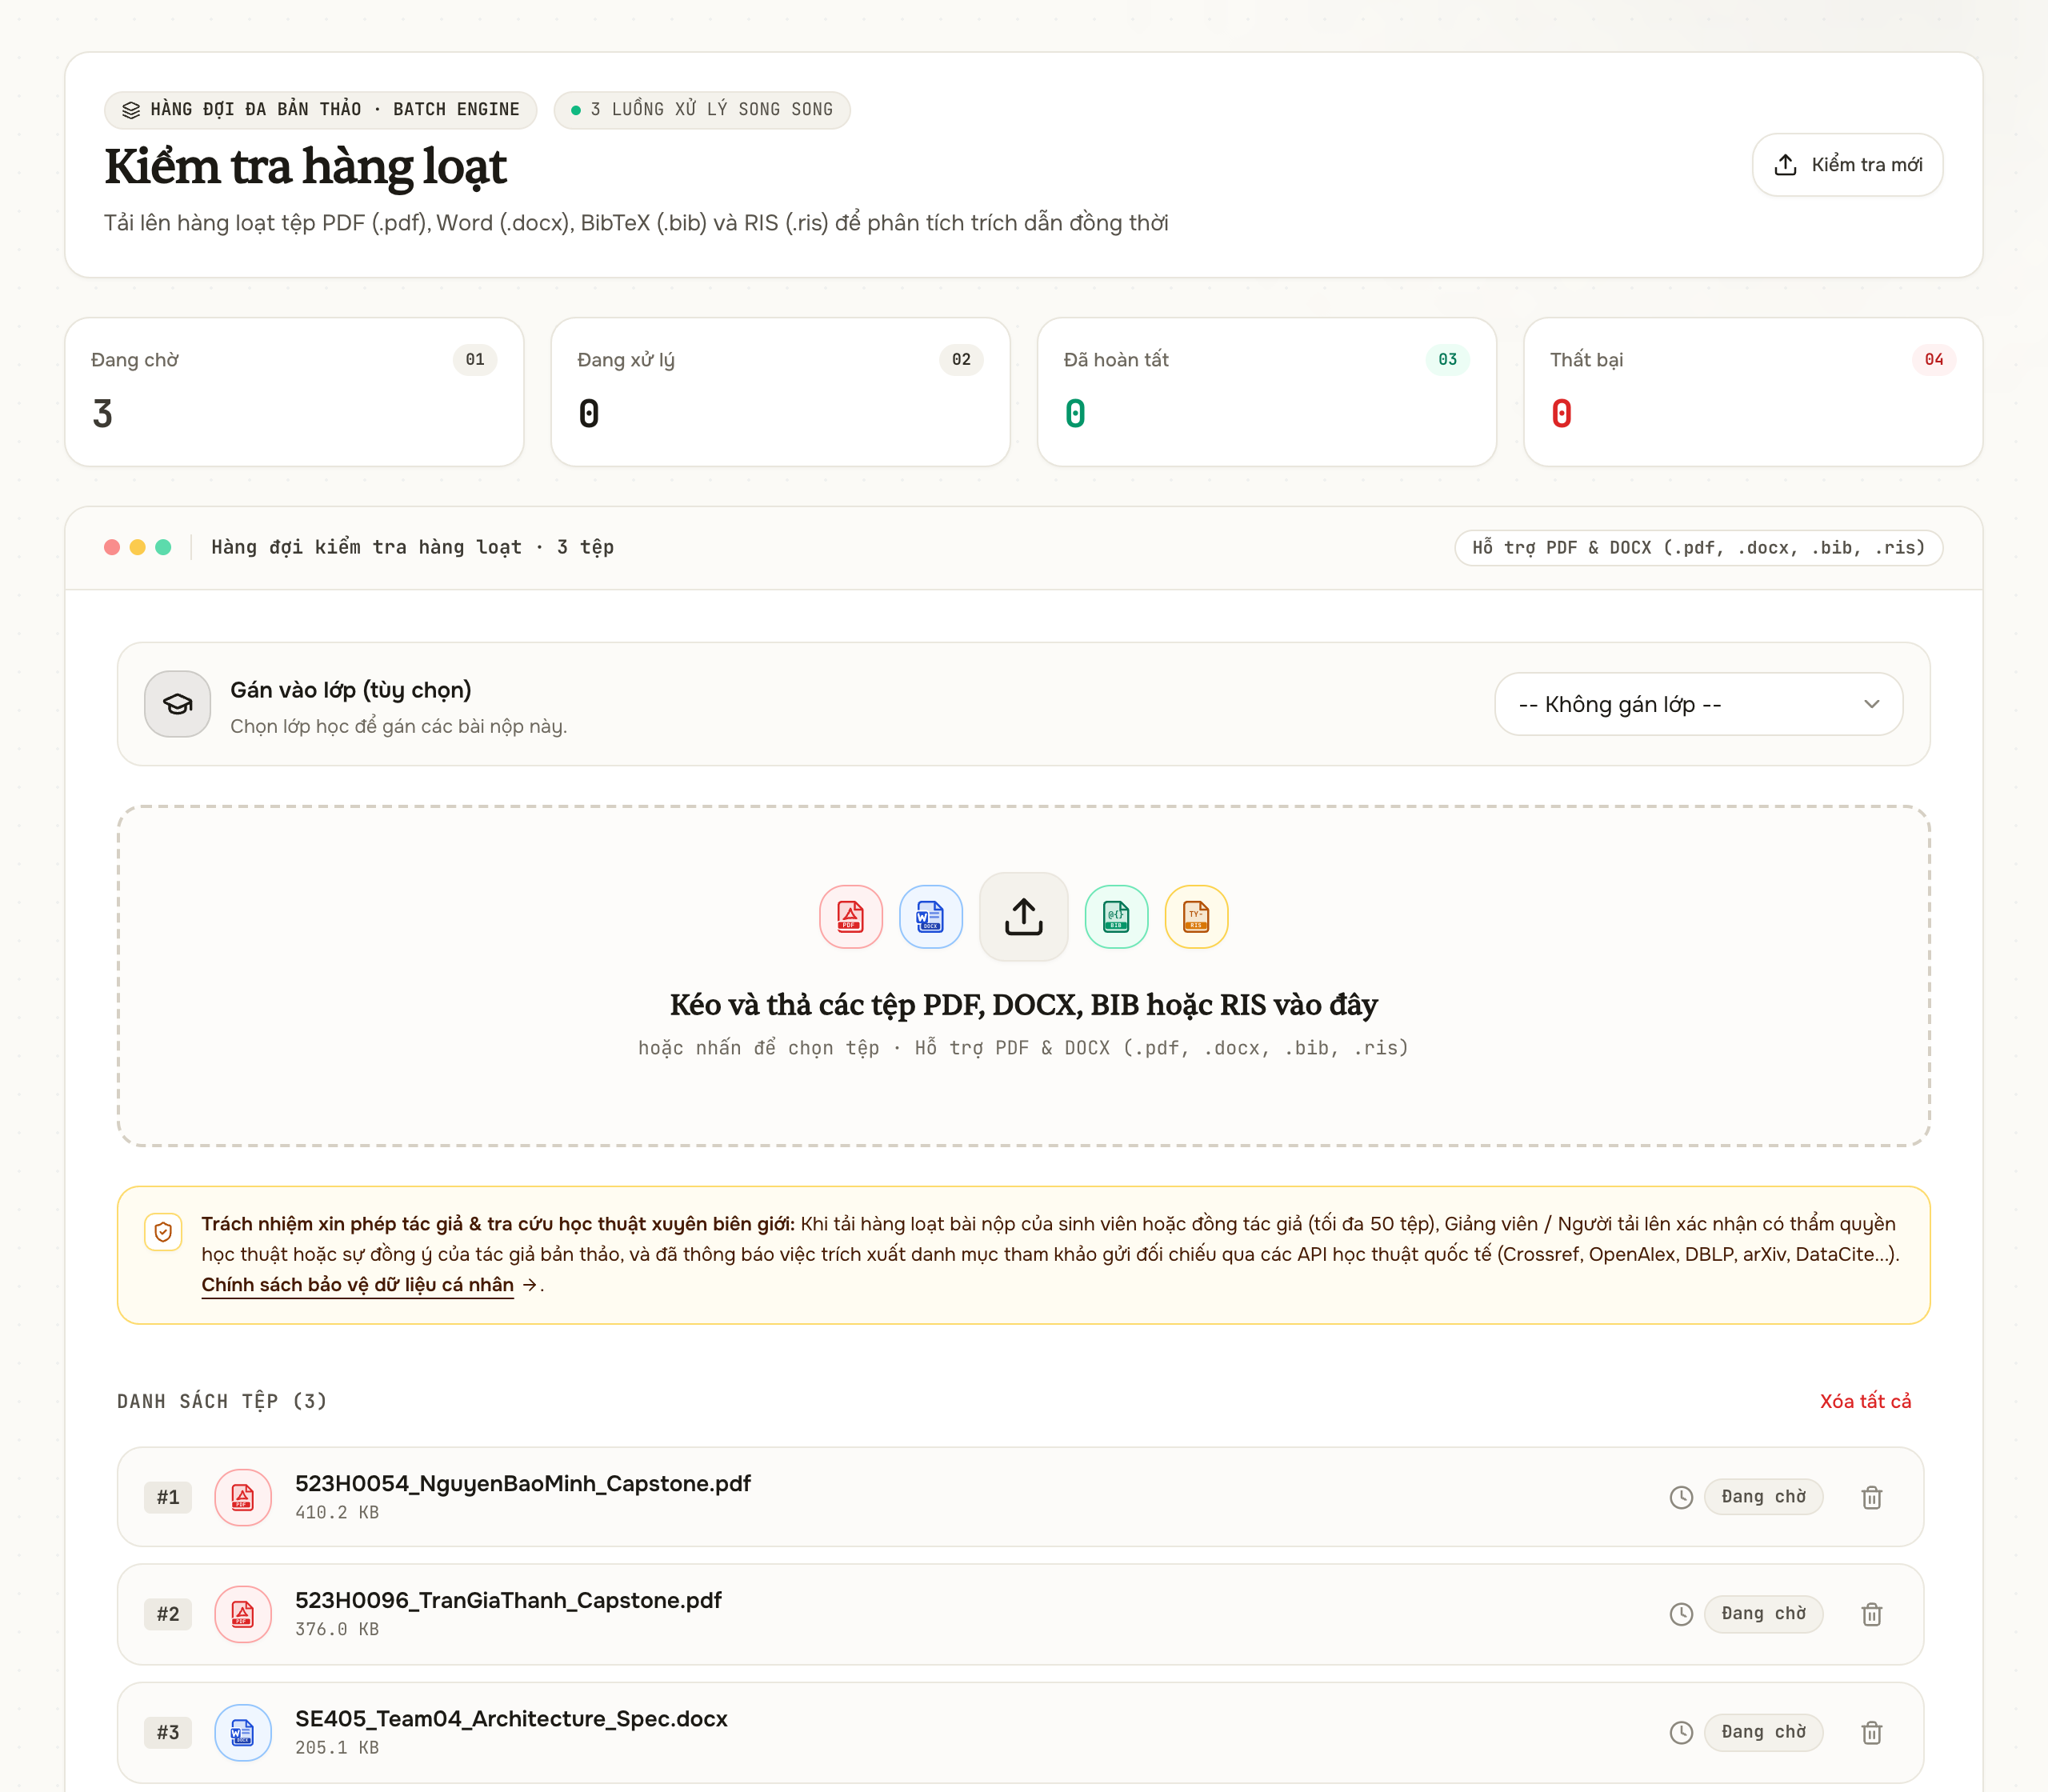
\includegraphics[width=0.94\textwidth,height=0.40\textheight,keepaspectratio]{picture/figures/04-batch-upload.png}}
    \caption[Bảng điều khiển sinh viên và hàng đợi tải lên hàng loạt đồng thời]{Bảng điều khiển kiểm chứng của sinh viên (\texttt{/dashboard}, trên) và hàng đợi kiểm chứng hàng loạt đa định dạng (\texttt{/batch-upload}, dưới), đã cắt thanh điều hướng trái để bảo đảm độ sắc nét trên khổ A4.}
    \label{fig:ui-workspace}
\end{figure}

\begin{figure}[!htbp]
    \centering
    \fboxsep=0pt\fboxrule=0.4pt\fbox{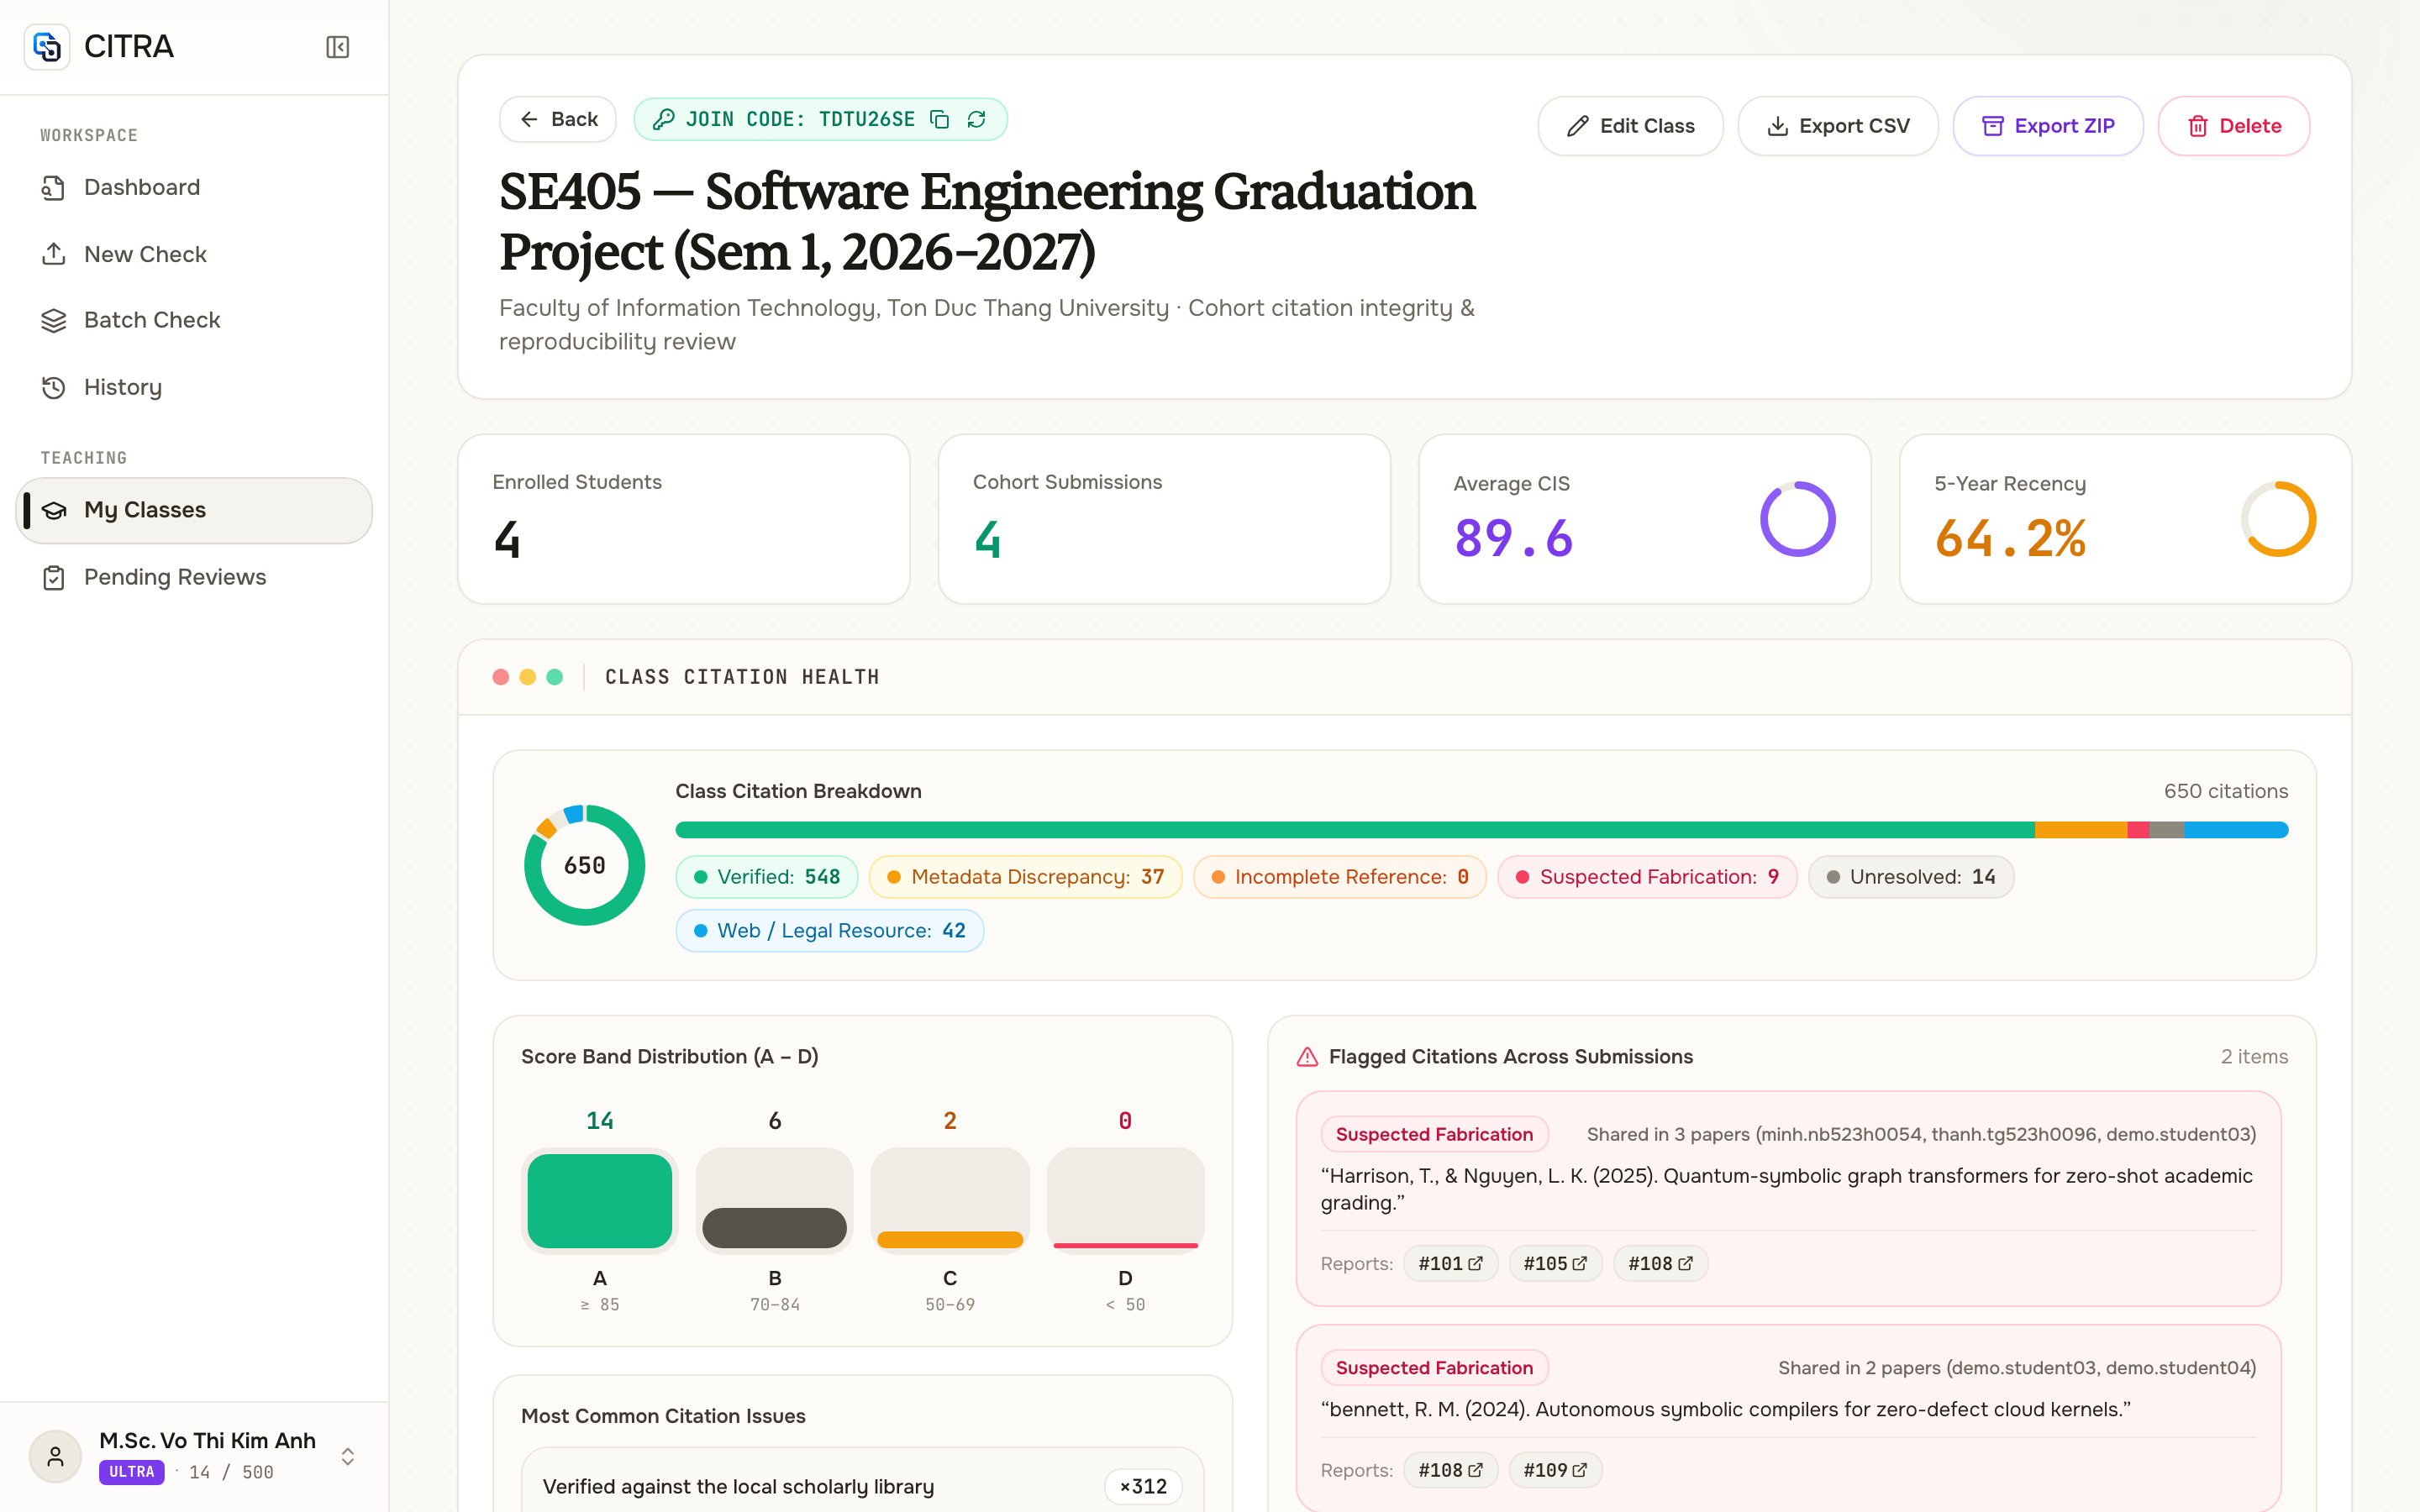
\includegraphics[width=0.94\textwidth,height=0.39\textheight,keepaspectratio]{picture/figures/10-teacher-classroom.png}}\\[6pt]
    \fboxsep=0pt\fboxrule=0.4pt\fbox{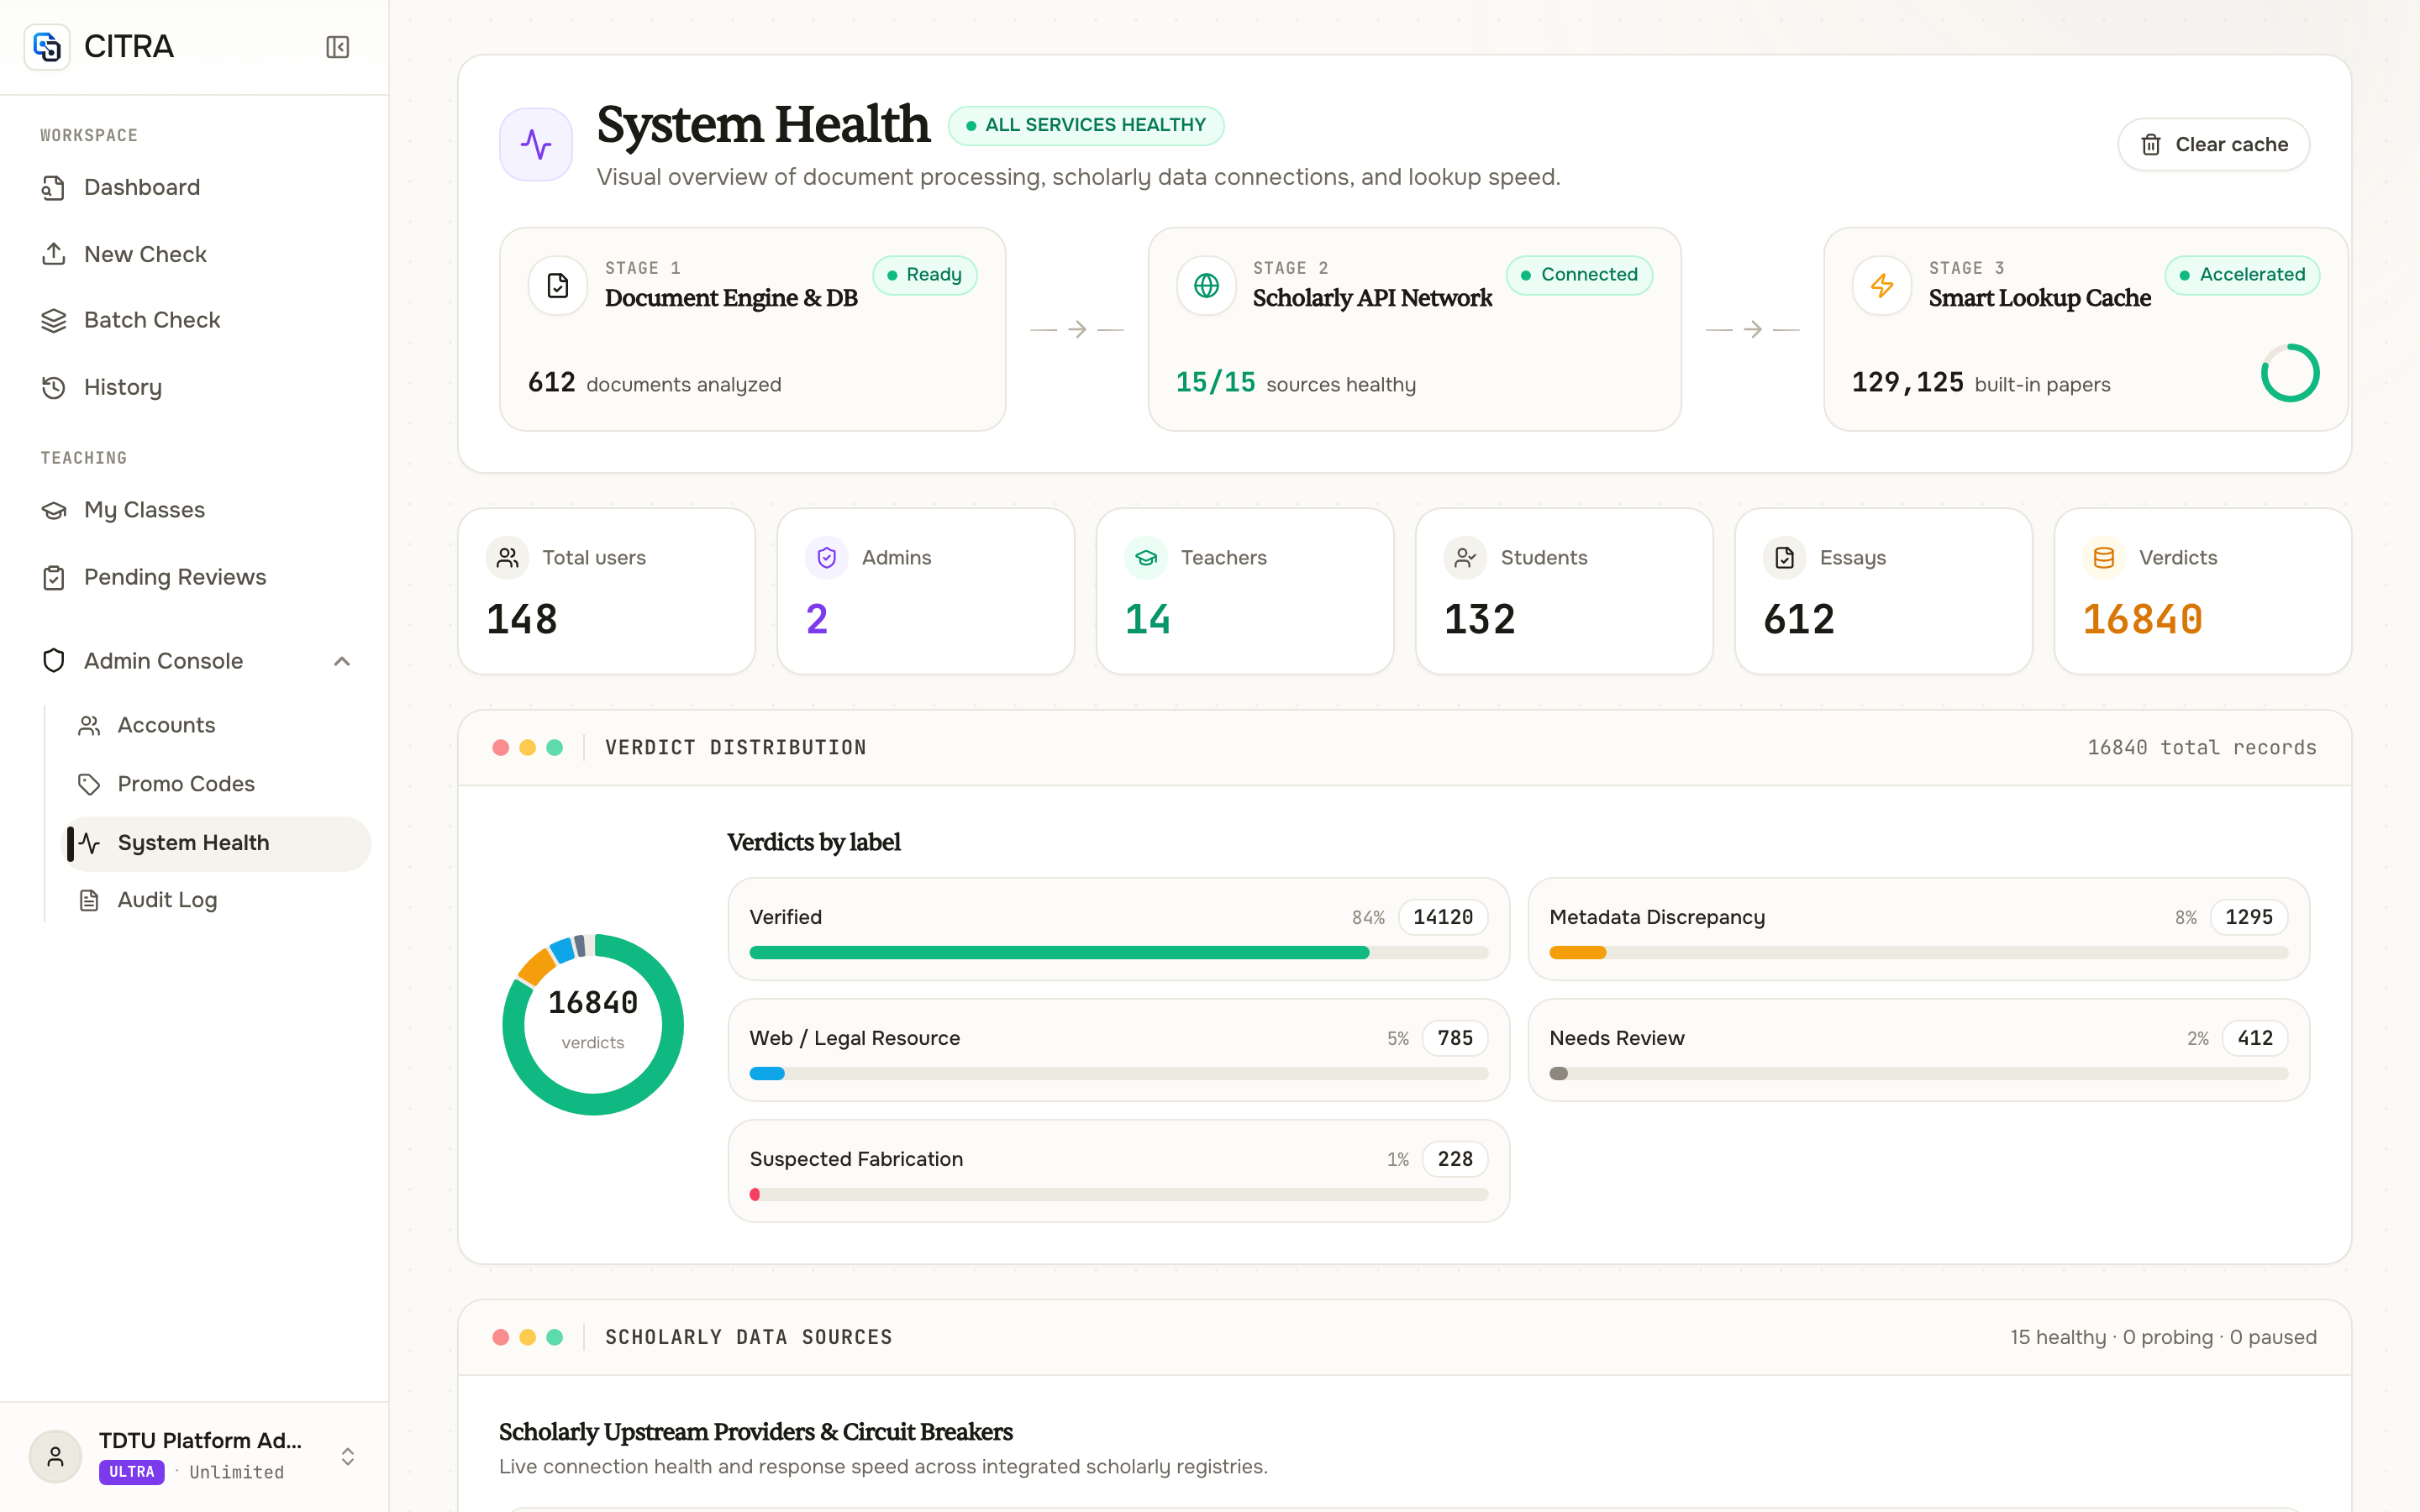
\includegraphics[width=0.94\textwidth,height=0.39\textheight,keepaspectratio]{picture/figures/11-admin-system-health.png}}
    \caption[Không gian phân tích lớp học của giảng viên và bảng giám sát hệ thống]{Giao diện phân tích lớp học của giảng viên (\texttt{/teacher/classes/1}, trên) và bảng giám sát hệ thống của quản trị viên hiển thị GROBID cùng các bộ ngắt mạch API (\texttt{/admin/system}, dưới).}
    \label{fig:ui-portals}
\end{figure}

\section{Tóm tắt chương}

Chương này đã trình bày kiến trúc nội tại và các thuật toán hình thức của \textbf{CITRA} xuyên suốt tám tầng: trích xuất mười hai định dạng, hợp nhất mức công trình và liên kết hai chiều bảy phương pháp (Thuật toán~\ref{alg:linker}), truy hồi bốn tầng với bảo vệ SSRF ghim IP, đối sánh ngữ nghĩa xuyên ngữ \texttt{VI}$\leftrightarrow$\texttt{EN} bằng bộ mã hóa kép, kiểm chứng lai Nơ-ron -- Ký hiệu 68 mã luật kết hợp Hồi quy Logistic 16 chiều và hiệu chỉnh Platt (Thuật toán~\ref{alg:verify} và Hình~\ref{fig:decision-flow}), công thức CIS năm thành phần đầy đủ cùng giao diện React 18.3 / TypeScript 5.9 tách gói tối ưu. Chương~\ref{chap:results} tiếp theo đánh giá thực nghiệm toàn bộ các thành phần này trên năm câu hỏi nghiên cứu.
